\documentclass[a4paper]{article}
\usepackage[utf8]{inputenc}

%=-=-=-=-=-=-=-=-=-=-=-=-=-=-=-=-=-=-=-=-=-=-=-=-=-=-=-=-=-=-=-=-=-=-=-=-=-=-=-=-
% PREAMBLE
%=-=-=-=-=-=-=-=-=-=-=-=-=-=-=-=-=-=-=-=-=-=-=-=-=-=-=-=-=-=-=-=-=-=-=-=-=-=-=-=-

%%%%%%%%%%%%%%%%%%%%%%%%%%%%%%%%%%%%%%%%%%%%%%%%%%%%%%%%%%%%%%%%%%%%%
% Important styling notes
%%
% For now, to include img.jpg in img/path/to/img.jpg, just use:
% path/to/img.jpg - for details see style.tex
%=-=-=-=-=-=-=-=-=-=-=-=-=-=-=-=-=-=-=-=-=-=-=-=-=-=-=-=-=-=-=-=-=-=-=-=-=-=-=-=-
% Packages
%%
%\usepackage{fullpage} % Package to use full page
\usepackage[top=1in,bottom=1in,left=1in,right=1in,heightrounded]{geometry}

\usepackage{parskip}                    % Package to tweak paragraph skipping
\usepackage{amsmath}                    % standard
\usepackage{amssymb}                    % standard - Double R symbol etc.
\usepackage{hyperref}
\usepackage{amsthm}                     % standard - theorem, definition, etc.
\usepackage{multicol}                   % multiple columns for numbering
\usepackage{enumitem}                   % standard - enumerate styles
\usepackage[utf8]{inputenc}
\usepackage{scrextend}                  % indentation
\usepackage{graphicx}                   % standard - add figures
\usepackage{float}                      % standard - figure position, use [H] option
\usepackage{pifont}                     % symbols http://willbenton.com/wb-images/pifont.pdf
                                        % e.g. \ding{51}
\usepackage{gensymb}                    % degree symbol \degree
\usepackage{xcolor}                     % bg color
\hypersetup{
    colorlinks,
    linkcolor={black!50!black},
    citecolor={blue!50!black},
    urlcolor={blue!80!black}
}
\usepackage{framed}                     % bg color
\usepackage[T1]{fontenc}                % small caps
\usepackage{sectsty}                    % headings colour
\usepackage{mathtools}                  % Loads amsmath
\usepackage{amsthm,thmtools,xcolor}     % coloured theorem
\usepackage[toc,page]{appendix}         % reference to appendix
%\usepackage{titlesec}                   % change chapter, section, etc. formats
\usepackage{xifthen}                    % if, else
\usepackage{etoolbox}
% format numbering in theorem, lemma, etc. environment
\AtBeginEnvironment{theorem}{\setlist[enumerate, 1]{font=\upshape,  wide=0.5em, before=\leavevmode}}
\AtBeginEnvironment{lemma}{\setlist[enumerate, 1]{font=\upshape,  wide=0.5em, before=\leavevmode}}
\usepackage[letterspace=150]{microtype} % \textls{<letterspaced text>} % 0 <= letterspace <= 1000, 1000 = M space
\usepackage{letltxmacro}                % renew commands?
\usepackage{minted}                     % package to list code
    % otherwise minted goes off the page
    \setmintedinline{breaklines}
\usepackage{subfig}
\usepackage{eso-pic}                    % title page bg pic
\usepackage{varwidth}
\PassOptionsToPackage{svgnames}{xcolor}
\usepackage{fontawesome}                % \faQuestionCircle
\usepackage{marvosym}                   %\Pointinghand
\usepackage{mdframed}                   % easy outline frames
\usepackage[many]{tcolorbox}            % colour box for theorem styles
\usepackage{array,booktabs,calc} % table figs and text
\usepackage{comment}                    % \begin{comment}
\usepackage{fancyhdr}                   % page headings
\usepackage{mdframed}                   % boxes
\usepackage[backend=biber,sorting=none,style=ieee]{biblatex}
\usepackage{caption}
%%% caption options {
%\DeclareCaptionFont{white}{\color{white}}
\DeclareCaptionFormat{listing}{\colorbox{magenta!30!gray}{\parbox{\textwidth}{#1#2#3}}}
\captionsetup[lstlisting]{format=listing,labelfont={bf,small},textfont=small,skip=-1pt}
%%% }
\addbibresource{bibliography.bib}
\usepackage{url}
\usepackage{textcomp}
\usepackage[makeroom]{cancel}           % crossed symbols - \cancel{}, \bcancel{}, xcancel{}
\usepackage{algorithm}
\usepackage[noend]{algpseudocode}
\usepackage{tikz}
\usetikzlibrary{arrows.meta,positioning,quotes} % arrows and nodes in tikz
\usepackage{marginnote}                 % things in page margin by \marginnote{...}
\usepackage{pgfplots}
\usepackage{pstricks-add,pst-slpe}      % for fancy tikz arrows
%\usepackage{titlesec}                  % title style
\usepackage{lmodern}                    % a font
\usepackage{titletoc}                   % Required for manipulating the table of contents
\usepackage{titlesec}                   % Allows customization of titles
\usepackage{fouriernc}                  % Use the New Century Schoolbook font
\usepackage{booktabs}                   % better tables
\usepackage{stmaryrd }                  % \varoast
\usepackage{listings}                   % code listings
\usepackage{longtable}                  % table across multiple pages
\usepackage{todonotes}                  % TODO bubbles by \todo{...} command
\usepackage{changepage}                 % paragraph margins
\usepackage{tikz}
\usetikzlibrary{calc}
\usepackage{eso-pic}
\usepackage{transparent}
\usepackage[makeroom]{cancel}

%=-=-=-=-=-=-=-=-=-=-=-=-=-=-=-=-=-=-=-=-=-=-=-=-=-=-=-=-=-=-=-=-=-=-=-=-=-=-=-=-
% Colours for various things
%%


\definecolor{shadecolor}{rgb}{1.,0.933,0.96} % bg color, r,g,b <= 1
\definecolor{medium_blue}{RGB}{60,125,190}
\definecolor{dark_blue}{RGB}{25,60,85}
\definecolor{dark_red}{RGB}{77,16,16}
\definecolor{LightPink}{rgb}{0.92.,0.8,0.84} % bg color, r,g,b <= 1
\definecolor{LighterPink}{rgb}{1.,0.94,0.97} % bg color, r,g,b <= 1
\definecolor{LightestPink}{rgb}{1.,0.95,0.99} % bg color, r,g,b <= 1
\definecolor{DarkestPink}{rgb}{0.36, 0.0, 0.18}
\definecolor{DarkerPink}{rgb}{0.41, 0.0, 0.21}
\definecolor{DarkPink}{rgb}{0.55, 0.05, 0.37}
\definecolor{lightestestpink}{RGB}{255,248,252}
\definecolor{codegray}{rgb}{0.5,0.5,0.5}
\definecolor{codegrayblue}{rgb}{0.35,0.35,0.47}



%=-=-=-=-=-=-=-=-=-=-=-=-=-=-=-=-=-=-=-=-=-=-=-=-=-=-=-=-=-=-=-=-=-=-=-=-=-=-=-=-
% Define my own theorem styles
%%

% "base" styles
\declaretheoremstyle[
  headfont=\color{DarkPink}\bfseries,
  bodyfont=\itshape,
]{colored}

\declaretheoremstyle[
  headfont=\color{DarkPink}\bfseries,
  bodyfont=\normalfont,
]{colored_upright}

% theorems (corollaries, etc) themselves, inherit from my style above
% Usage:
% \begin{theorem} \end{theorem}, \begin{lemma} \end{lemma}, ...
\declaretheorem[
	numberwithin=section,
 	style=colored,
	name=\textsc{Theorem},
]{theorem}

\tcolorboxenvironment{theorem}{
  boxrule=0pt,
  boxsep=2pt,
  colback={magenta!25!white},
  colframe=DarkPink,
  enhanced jigsaw, 
  borderline west={2pt}{0pt}{DarkPink},
  sharp corners,
  before skip=5pt,
  after skip=5pt,
  breakable,
  right=0mm % for equations
}

\declaretheorem[
	numberwithin=section,
 	style=colored,
	name=\textsc{Corollary},
]{corollary}

\tcolorboxenvironment{corollary}{
  boxrule=0pt,
  boxsep=1pt,
  colback={magenta!10!white},
  colframe=DarkPink,
  enhanced jigsaw, 
  borderline west={2pt}{0pt}{DarkPink},
  sharp corners,
  before skip=5pt,
  after skip=5pt,
  breakable,
  right=0mm % for equations
}

\declaretheorem[
	numberwithin=section,
	style=colored,
	name=\textsc{Lemma},
]{lemma}

\tcolorboxenvironment{lemma}{
  boxrule=0pt,
  boxsep=1pt,
  colback={magenta!10!white},
  colframe=DarkPink,
  enhanced jigsaw, 
  borderline west={2pt}{0pt}{DarkPink},
  sharp corners,
  before skip=5pt,
  after skip=5pt,
  breakable,
  right=0mm % for equations
}

\declaretheorem[
	numberwithin=section,
	style=colored,
	name=\textsc{Definition},
]{definition}

\tcolorboxenvironment{definition}{
  boxrule=0pt,
  boxsep=1pt,
  colback={magenta!25!white},
  colframe=DarkPink,
  enhanced jigsaw, 
  borderline west={2pt}{0pt}{DarkPink},
  sharp corners,
  before skip=5pt,
  after skip=5pt,
  breakable,
  right=0mm % for equations
}

\declaretheorem[
	numberwithin=section,
  	style=colored,
  	name=\textsc{Example},
]{exmp}

\declaretheorem[
	numberwithin=section,
  	style=colored,
  	name=\textsc{Solution},
]{soln}

%%% code listings
\lstdefinestyle{code1}{
    backgroundcolor=\color{lightestestpink},   
    commentstyle=\color{codegrayblue},
    keywordstyle=\color{DarkerPink},
    numberstyle=\tiny\color{codegray},
    stringstyle=\color{black!40!cyan},
    basicstyle=\small\ttfamily,
    breakatwhitespace=false,
    breaklines=true,        
    captionpos=t,             
    keepspaces=true,        
    numbers=left,           
    numbersep=5pt,
    showspaces=false, 
    showstringspaces=false,
    showtabs=false,
    tabsize=4
}

%%% code listings
\lstdefinestyle{code1}{
    backgroundcolor=\color{lightestestpink},   
    commentstyle=\color{codegrayblue},
    keywordstyle=\color{DarkerPink},
    numberstyle=\tiny\color{codegray},
    stringstyle=\color{black!40!cyan},
    basicstyle=\small\ttfamily,
    breakatwhitespace=false,
    breaklines=true,        
    captionpos=t,             
    keepspaces=true,        
    numbers=left,           
    numbersep=5pt,
    showspaces=false, 
    showstringspaces=false,
    showtabs=false,
    tabsize=4
}


\lstdefinestyle{terminal}{
    backgroundcolor=\color{black!5},   
    commentstyle=\color{codegrayblue},
    keywordstyle=\color{DarkerPink},
    %numberstyle=\tiny\color{codegray},
    stringstyle=\color{black!40!cyan},
    basicstyle=\small\ttfamily,
    numbers=none,
    breakatwhitespace=false,
    breaklines=true,        
    %captionpos=t,             
    keepspaces=true,        
    %numbers=left,           
    %numbersep=5pt,
    showspaces=false, 
    showstringspaces=false,
    showtabs=false,
    tabsize=4
}

\lstset{style=code1}

%=-=-=-=-=-=-=-=-=-=-=-=-=-=-=-=-=-=-=-=-=-=-=-=-=-=-=-=-=-=-=-=-=-=-=-=-=-=-=-=-
% Headers (size, font, colour)
%%

\makeatletter
\renewcommand{\@seccntformat}[1]{\llap{\textcolor{DarkestPink}{\csname the#1\endcsname}\hspace{1em}}}                    
\renewcommand{\section}{\@startsection{section}{1}{\z@}
{-4ex \@plus -1ex \@minus -.4ex}
{1ex \@plus.2ex }
{\normalfont\large\sffamily\bfseries\textcolor{DarkestPink}}}
\renewcommand{\subsection}{\@startsection {subsection}{2}{\z@}
{-3ex \@plus -0.1ex \@minus -.4ex}
{0.5ex \@plus.2ex }
{\normalfont\sffamily\bfseries\textcolor{DarkestPink}}}
\renewcommand{\subsubsection}{\@startsection {subsubsection}{3}{\z@}
{-2ex \@plus -0.1ex \@minus -.2ex}
{.2ex \@plus.2ex }
{\normalfont\small\sffamily\bfseries\textcolor{DarkestPink}}}                        


%=-=-=-=-=-=-=-=-=-=-=-=-=-=-=-=-=-=-=-=-=-=-=-=-=-=-=-=-=-=-=-=-=-=-=-=-=-=-=-=-
% Numberings, counters and spacings
%%
\numberwithin{equation}{section} % section number in eq/s
\setlength{\jot}{7pt} % spacing in split, gathered env/s



%% Custom examples
%% Output - Example 1,2,...
\newcounter{example}
\newenvironment{example}[1][]{\refstepcounter{example}\par\medskip
   \textbf{Example~\theexample. #1} \rmfamily}{\medskip}
%%%%%%%%%%%% End of unused %%%%%%%%%%%%



%=-=-=-=-=-=-=-=-=-=-=-=-=-=-=-=-=-=-=-=-=-=-=-=-=-=-=-=-=-=-=-=-=-=-=-=-=-=-=-=-
% Paths
%%

%=-=-=-=-=-=-=-=-=-=-=-=-=-=-=-=-=-=-=-=-=-=-=-=-=-=-=-=-=-=-=-=-=-=-=-=-=-=-=-=-
% User defined macros (math mode)
%%


% Curly braces under text. Usage: \myunderbrace{upper}{lower}
\newcommand{\myunderbrace}[2]{\mathrlap{\underbrace{\phantom{#1}}_{#2}} #1}
\newcommand{\setR}{\mathbb{R}} % \ouble R
\newcommand{\setRn}{\mathbb{R}^n} %  double R^n
\newcommand{\setN}{\mathbb{N}} % double N
\newcommand{\setZ}{\mathbb{Z}} % double Z
\let\oldemptyset\emptyset
\let\emptyset\varnothing % nice - looking empty set symbol
\newcommand{\fancyN}{\mathcal{N}} % null space
\newcommand{\fancyR}{\mathcal{R}} % range

\newcommand{\ba}{\textbf{a}}
\newcommand{\be}{\textbf{e}}
\newcommand{\bw}{\textbf{w}}
\newcommand{\bx}{\textbf{x}}
\newcommand{\bu}{\textbf{u}}
\newcommand{\bv}{\textbf{v}}
\newcommand{\by}{\textbf{y}}
\newcommand{\bz}{\textbf{z}}
\newcommand{\bb}{\textbf{b}}
\newcommand{\bA}{\textbf{A}}
\newcommand{\bB}{\textbf{B}}
\newcommand{\bC}{\textbf{C}}
\newcommand{\bD}{\textbf{C}}
\newcommand{\bI}{\textbf{I}}
\newcommand{\bM}{\textbf{M}}
\newcommand{\bO}{\textbf{0}}
\newcommand{\bS}{\textbf{S}}
\newcommand{\bX}{\textbf{X}}
\newcommand{\bU}{\textbf{U}}
\newcommand{\bY}{\textbf{Y}}
% double bars as in norm
%\newcommand{\norm}[1] {\left|\left| #1 \right| \right|} 
\newcommand{\norm}[1]{\left\lVert#1\right\rVert}
\renewcommand{\t}{^{\top}}

\newcommand{\mean}[1]{\bar{#1}}
\newcommand{\var}{\sigma^2}

\newcommand{\partdevx}[1]{\frac{\partial #1}{\partial x}}
\newcommand{\partdevt}[1]{\frac{\partial #1}{\partial t}}
\newcommand{\partdevxx}[1]{\frac{\partial #1}{\partial x}}
\newcommand{\partdevxn}[1]{\frac{\partial^n #1}{\partial x^n}}
\newcommand{\partdevy}[1]{\frac{\partial #1}{\partial y}}
\newcommand{\partdevyy}[1]{\frac{\partial #1}{\partial y}}
\newcommand{\partdevyn}[1]{\frac{\partial^n #1}{\partial y^n}}

% text above = symbol
\newcommand{\overeq}[1]{\ensuremath{\stackrel{#1}=}} 
\newcommand{\greatersmaller}{%
  \mathrel{\ooalign{\raisebox{.6ex}{$>$}\cr\raisebox{-.6ex}{$<$}}}
} % greater and smaller symbols on top of each other, same line

%=-=-=-=-=-=-=-=-=-=-=-=-=-=-=-=-=-=-=-=-=-=-=-=-=-=-=-=-=-=-=-=-=-=-=-=-=-=-=-=-
% User defined macros (non math)

\newcommand{\qedblack}{$\hfill\blacksquare$} % black square end of line
\newcommand{\qedwhite}{\hfill \ensuremath{\Box}} % white square end of line
\newcommand{\hquad}{\hskip0.5em\relax}% half quad space
%\newcommand{\TODO}{\textcolor{red}{\bf TODO!}\;}

\newcommand{\TODO}[1][]{%
    \ifthenelse{\equal{#1}{}}{\textcolor{red}{\bf TODO!}\;}{\textcolor{red}{\textbf {TODO:} #1}\; }%
}
\newcommand{\B}[1]{\textbf{\textup{#1}}} % bold and upright
\renewcommand{\labelitemi}{\scriptsize$\textcolor{DarkPink}{\blacksquare}$} % itemize - squares instead of bullets
\newcommand{\emphasis}[1]{\textls{#1}}

\LetLtxMacro{\originaleqref}{\eqref}
\renewcommand{\eqref}{Eq.~\originaleqref}
\renewcommand*{\eqref}[1]{Eq.~\originaleqref{#1}}





% background images
%%%%%%%
\newcommand\BackgroundPic{%
\put(0,0){%
\parbox[b][\paperheight]{\paperwidth}{%
\vfill
%\centering
\includegraphics[width=0.125\paperwidth,height=\paperheight,%
]{img/background_02.png}% use ,keepaspectratio
\vfill
}}}
%%%%%%%
% end of background image
%%%%%%%%%%%%%% my own frame
\newmdenv[topline=false,bottomline=false]{leftrightbox}
%%%%%%%%%%%%% end
%%%%%%%%%%%%% my own comment
\newcommand{\mycomment}[1]{\begin{leftrightbox}\Pointinghand~\textbf{Comment:}~#1 \end{leftrightbox}}
%%%%%%%%%%%%% end
% my custom note https://tex.stackexchange.com/questions/301993/create-custom-note-environment-with-tcolorbox
\newmdenv[
    topline=false,
    bottomline=false,
    rightline=false,
    innerrightmargin=0pt
]{siderule}
\newenvironment{mynote}%
    {\begin{siderule}\textbf{\Pointinghand~Note:}}
    {\end{siderule}}
    
\newenvironment{myquote}%
    {\begin{adjustwidth}{0.4cm}{0.4cm}\faQuoteLeft\ \itshape}
    { \hfill \faQuoteRight  \end{adjustwidth}}
%%%%%%%%%%%%% my own box
\newcommand{\boxone}[1]{\begin{tcolorbox}[colback = LighterPink,colframe=LightPink]
#1
\end{tcolorbox}}
\newcommand{\boxsimple}[1]{\begin{tcolorbox}[
	colback = white,
	colframe=black!70,
	coltitle = black!20,
	title    = {Problem},]
#1
\end{tcolorbox}}
%%%%%%%%%%%%% end

\newcommand{\bigtitle}[1]{\LARGE\textsc{{\textbf{#1}}}\normalsize\vspace{0.25cm}}

\let\oldemptyset\emptyset
\let\emptyset\varnothing
%algorithmic
\algdef{SE}[DOWHILE]{Do}{doWhile}{\algorithmicdo}[1]{\algorithmicwhile\ #1}%

%%% otherwise minted goes off the page
\setmintedinline{breaklines}




\begin{document}
%=-=-=-=-=-=-=-=-=-=-=-=-=-=-=-=-=-=-=-=-=-=-=-=-=-=-=-=-=-=-=-=-=-=-=-=-=-=-=-=-
% GLOBAL STYLES (DOCUMENT SCOPE)
%=-=-=-=-=-=-=-=-=-=-=-=-=-=-=-=-=-=-=-=-=-=-=-=-=-=-=-=-=-=-=-=-=-=-=-=-=-=-=-=-
% caption: Figure 1 -> <bold> Fig. 1 </bold>
\captionsetup[figure]{labelfont={bf},labelformat={default},labelsep=period,name={Fig.}}


%=-=-=-=-=-=-=-=-=-=-=-=-=-=-=-=-=-=-=-=-=-=-=-=-=-=-=-=-=-=-=-=-=-=-=-=-=-=-=-=-
% TITLE PAGE
%=-=-=-=-=-=-=-=-=-=-=-=-=-=-=-=-=-=-=-=-=-=-=-=-=-=-=-=-=-=-=-=-=-=-=-=-=-=-=-=-
%%%%%%%%%%%%%%%%%%%%%%%%%%%%%%%%%%%%%%%%%
% Formal Book Title Page
% LaTeX Template
% Version 2.0 (23/7/17)
%
% This template was downloaded from:
% http://www.LaTeXTemplates.com
%
% Original author:
% Peter Wilson (herries.press@earthlink.net) with modifications by:
% Vel (vel@latextemplates.com)
%
% License:
% CC BY-NC-SA 3.0 (http://creativecommons.org/licenses/by-nc-sa/3.0/)
% 
% This template can be used in one of two ways:
%
% 1) Content can be added at the end of this file just before the \end{document}
% to use this title page as the starting point for your document.
%
% 2) Alternatively, if you already have a document which you wish to add this
% title page to, copy everything between the \begin{document} and
% \end{document} and paste it where you would like the title page in your
% document. You will then need to insert the packages and document 
% configurations into your document carefully making sure you are not loading
% the same package twice and that there are no clashes.
%
%%%%%%%%%%%%%%%%%%%%%%%%%%%%%%%%%%%%%%%%%

%----------------------------------------------------------------------------------------
%	PACKAGES AND OTHER DOCUMENT CONFIGURATIONS
%----------------------------------------------------------------------------------------



%----------------------------------------------------------------------------------------
%	TITLE PAGE
%----------------------------------------------------------------------------------------



\begin{titlepage} % Suppresses headers and footers on the title page

	%------------------------------------------------
	%	Border decorations
	%------------------------------------------------
    \AddToShipoutPictureBG*{
        \begin{tikzpicture}[overlay,remember picture]
            \draw[line width=10pt]
                ($ (current page.north west) + (4pt,-4pt) $)
                rectangle
                ($ (current page.south east) + (4pt,4pt) $);
            \draw[line width=10pt]
                ($ (current page.north west) + (4pt,-4pt) $)
                rectangle
                ($ (current page.south east) + (-4pt,4pt) $);
        \end{tikzpicture}
        \AtTextUpperLeft{%
            \put(185,12){
                \parbox[b][\paperheight]{\paperwidth}{% parbox
            
                    \centering
                    {\transparent{1.0}
                    \setlength{\fboxsep}{0pt}%
                    \setlength{\fboxrule}{2pt}%
                    \fbox{                                
                        \includegraphics[keepaspectratio=false,width=50pt,height=50pt]{img/title/corner.png}
                        }
                    } % transparent
                } % parbox
            } % put
        } % AtTextUpperLeft
        
        \AtTextUpperLeft{%
            \put(185,-762){
                \parbox[b][\paperheight]{\paperwidth}{% parbox
            
                    \centering
                    {\transparent{1.0}
                    \setlength{\fboxsep}{0pt}%
                    \setlength{\fboxrule}{2pt}%
                    \fbox{                                
                        \includegraphics[keepaspectratio=false,width=50pt,height=50pt]{img/title/corner.png}
                        }
                    } % transparent
                } % parbox
            } % put
        } % AtTextUpperLeft
        
         \AtTextUpperLeft{%
            \put(-338,-762){
                \parbox[b][\paperheight]{\paperwidth}{% parbox
            
                    \centering
                    {\transparent{1.0}
                    \setlength{\fboxsep}{0pt}%
                    \setlength{\fboxrule}{2pt}%
                    \fbox{                                
                        \includegraphics[keepaspectratio=false,width=50pt,height=50pt]{img/title/corner.png}
                        }
                    } % transparent
                } % parbox
            } % put
        } % AtTextUpperLeft
        
        \AtTextUpperLeft{%
            \put(-338,12){
                \parbox[b][\paperheight]{\paperwidth}{% parbox
            
                    \centering
                    {\transparent{1.0}
                    \setlength{\fboxsep}{0pt}%
                    \setlength{\fboxrule}{2pt}%
                    \fbox{                                
                        \includegraphics[keepaspectratio=false,width=50pt,height=50pt]{img/title/corner.png}
                        }
                    } % transparent
                } % parbox
            } % put
        } % AtTextUpperLeft
    } %AddToShipoutPictureBG
    
    
   	%------------------------------------------------
	%	Text alignment
	%------------------------------------------------
	\centering % Centre everything on the title page
	
	\scshape % Use small caps for all text on the title page
	
	\vspace*{\baselineskip} % White space at the top of the page
	
	%------------------------------------------------
	%	Title
	%------------------------------------------------
	
	\rule{\textwidth}{1.6pt}\vspace*{-\baselineskip}\vspace*{2pt} % Thick horizontal rule
	\rule{\textwidth}{0.4pt} % Thin horizontal rule
	
	\vspace{0.75\baselineskip} % Whitespace above the title
	
	{\LARGE NOTES ON\\ \Large 3D GEOMETRY FOR COMPUTER VISION\\ \Large AND SLAM} % Title
	
	\vspace{0.75\baselineskip} % Whitespace below the title
	
	\rule{\textwidth}{0.4pt}\vspace*{-\baselineskip}\vspace{3.2pt} % Thin horizontal rule
	\rule{\textwidth}{1.6pt} % Thick horizontal rule
	
	\vspace{2\baselineskip} % Whitespace after the title block
	
	%------------------------------------------------
	%	Subtitle
	%------------------------------------------------
	Contents
	
	\vspace*{3\baselineskip} % Whitespace under the subtitle
	
	Projective Geometry\\
	Image Rectification\\
	SLAM
	
	\vspace*{3\baselineskip} % Whitespace under the subtitle
	
	%------------------------------------------------
	%	Editor(s)
	%------------------------------------------------
	
	By
	
	\vspace{0.5\baselineskip} % Whitespace before the editors
	
	{\normalfont \Large \mintinline{latex}{0xLeo} (\url{github.com/0xleo}) \\} % Editor list
	
	\vspace{0.5\baselineskip} % Whitespace below the editor list
	
	%\textit{The University of California \\ Berkeley} % Editor affiliation
	
	\vfill % Whitespace between editor names and publisher logo
	
	%------------------------------------------------
	%	Publisher
	%------------------------------------------------
	
	
	\vspace{0.3\baselineskip} % Whitespace under the publisher logo
	
	\today % Date
	
	{DRAFT X.YY} % Draft version
	{\\Missing: \ldots}

\end{titlepage}

%----------------------------------------------------------------------------------------
%\maketitle



%=-=-=-=-=-=-=-=-=-=-=-=-=-=-=-=-=-=-=-=-=-=-=-=-=-=-=-=-=-=-=-=-=-=-=-=-=-=-=-=-
% MAIN DOCUMENT
%=-=-=-=-=-=-=-=-=-=-=-=-=-=-=-=-=-=-=-=-=-=-=-=-=-=-=-=-=-=-=-=-=-=-=-=-=-=-=-=-
\newpage
\tableofcontents
\newpage

\section{Histogram-Based Methods}

\subsection{Histogram backprojection}

\subsubsection{Intuition - model and search image histogram}
In image processing, we are usually interested in histograms of greyscale images. However, often the colour histogram can be used to identify an image region or object. RGB histograms are practically not good enough for matching as the R, G, B components are strongly correlation with the illumination hitting the object. In practice, objects are converted from RGB to HSV (Hue, Saturation, Value) domain. \emphasis{Hue} represents the colour type (blue, yellow, etc.), \emphasis{saturation} represents the vibrancy (how vivid or neutral it is) and \emphasis{value} represents the brightness of the colour. Hence HSV decouples the brightness from the colour description. Therefore when performing colour matching we are only interested in the H and S components, which map to a 2D histogram. More about the HSV domain in \ref{app:hsv_domain}.

\mycomment{
The HS components are often but \textit{not always} a good choice for colour-based detection. They may fail detecting black and white objects since black and white can have any colour (H) and in this case the SV components of the HSV or even the YUV domain are a better choice. However, in this article we stick to HS.
}

\emphasis{Histogram backprojection} answers the question ``where in the image are the colours that belong to the object being looked for?''. We do this by defining a \emphasis{model} image (the object we search for -- a. k.a. \emphasis{target}) and the \emphasis{search} (the whole image where we search in), probing the model over search image and calculating their histogram  similarity at each position.

Just to illustrate the idea, assume that we want to match the greyscale (instead of the 2D) histogram of the garlic in Fig. \ref{fig:peppers_and_garlic}. A part of the top garlic has been chosen as the model. The histogram of the model is shown as well as that of two matching candidates. In this case, the histogram of ``match 2'' is more similar to the model's than one ``match 1'' so we want somehow to register that similarity. The question attempted to be answered in the next section is ``how do we measure the similarity of the histogram of the matching candidate to that of the model?''.
\begin{figure}[H]
    \centering
    \includegraphics[height=6.5cm]{img/image_hist_different_regions.png}
    \caption{Model and two matches' greyscale histograms.}
    \label{fig:peppers_and_garlic}
\end{figure}


\subsubsection{(optional) The rationale behind defining the ratio histogram}

We assume that 
\begin{enumerate}
    \item the model's histogram (the object we search for) is narrow and tall
    \item and the scene's (whole input image) histogram is rather wide.
\end{enumerate}
It has then been proven (it won't be discussed in this article how as the how is out of scope) that a good histogram similarity measure between the model $M$ and a patch of the image we search it in $I$ is the ratio histogram $R$. $M$ and $I$ need to be pre-calculated and can be divided element-wise, since they have the same range and bins to obtain $R$. The \emphasis{ratio histogram} is a therefore function $R:\mathbb{Z}^2 \rightarrow \mathbb{R}$ that maps a colour $(h,s)$ to some value. If $M(h,s) > I(h,s) \Rightarrow R(h,s) > 1$ that means the model has more pixels of colour $(h,s)$ relative to its total number of pixels compared to $I(h,s)$, and vice versa. If $R(h,s) = 1$, then that means  that the input and model images contain $(h,s)$ at the same degree.

However, because of assumptions (1), (2), $M(h,s) > I(h,s)$ can happen quite often and so long as $M(h,s) > I(h,s) \Rightarrow R(h,s)>1$, e.g. $R(h,s) = 2,3,10$, the exact value does not give much useful information. To summarise, $R$ de-emphasises pixels with colours that do not belong to the model and emphasises the rest.


\subsubsection{A colour matching heuristic}

From the previous section, the conclusion is that it is desirable to clip the ratio histogram to 1, as defined by Swain et al. 
\begin{definition}
For each bin $j$, the ratio histogram is defined as
\begin{equation}
    R_j = \min\left(\frac{M_j}{I_j},1\right)
\end{equation}
, where $M$, $I$ are the model's and input's histograms respectively.
\end{definition}
Note that $j$ does not necessarily have to be a pair $(h,s)$, but it if a histogram bin (index) is quantised it can be a rectangle in the 2D space, such as $[20, 39] \times [50, 69]$. As mentioned before, $R$ associates a colour with its probability of appearing in the model and the next step is the associate each pixel with that probability.

Each pixel of the original image at $(x,y)$ maps to a 2D HS value, by a colour function $c: \mathbb{Z}^2 \leftarrow \mathbb{Z}^2$, by taking $c(x,y)$. Sometimes need an intermediate function $h:\mathbb{Z}^2 \rightarrow \mathbb{Z}^2$ that takes the output of $c$ and quantises it (groups multiple colours in one bin), before it is fed to $R$. For example, $h$ could convert $[0,1,\ldots,179] \times [0,1,\ldots,255]$ to $[0, 19, 39, \ldots,179] \times [0, 24, 49, \ldots, 255]$. The output of $h$ is bed to $R$, which divides $M_j$ to $I_j$ at each bin $j$.To summarise this paragraph we have  defined the following functions in backpropagation:
\begin{itemize}
    \item $c: \mathbb{Z}^2 \rightarrow \mathbb{Z}^2$: maps a pixel at $(x,y)$ to an HS value $(h_j,s_j)$.
    \item $h: \mathbb{Z}^2 \rightarrow \mathbb{Z}^2$ maps a set of values $(h_i,s_i,h_{i+1},s_{i+1},\ldots,h_n,s_n)$ to another $(h,s)$ value by having quantised the range of $h$ and $s$.
    \item $R: \mathbb{Z}^2 \rightarrow [0,1]$ maps an $(h,s)$ value to a probablity.
\end{itemize}
We therefore want to create a new image $b$ where each pixel $(x,y)$ gets assigned its output of $R$ - the measure of how much its colour appears in the model image. 
\begin{equation}
    b(x,y) := R\left(h\left(c(x,y)\right)\right)=
    \min\left(\frac{M\left(h\left(c(x,y)\right)\right)}{I\left(h\left(c(x,y)\right)\right)},1\right) \; \forall \; x,y
\end{equation}
The final step is to find compact regions where $b$ is high. If the shape of the object (model) to detect is generic, then this can be done by convolving $b$ with binary disk mask $D^r$ of radius $r$. Define:
\begin{equation}
    D_{x,y}^r = \left\{
\begin{array}{ll}
      1 & \sqrt{x^2+y^2} \leq r \\
      0 & \textup{otherwise}\\
\end{array} 
\right. 
\end{equation}
Then the probability image $b$ can be convolved with the mask:
\begin{equation}
    b := D^r \ast b
\end{equation}
The $\arg \max$ function to returns the pixel $(x, y)$ with
the maximum value of its argument, i.e. of the $R$ matrix and the $\ast$ symbol denotes convolution. Then Histogram Backprojection algorithm can be then
written
\begin{algorithm}[H]
\caption{Colour matching by histogram backprojection according to Swain et al}
\label{alg:hist_backproj}
\begin{algorithmic}[1]
\Procedure{Hist-BackProj} {ImM, ImI} \Comment{ImM: model, ImI: search image}
\State $M\leftarrow \textup{histogram}(ImM)$
\State $I\leftarrow \textup{histogram}(ImI)$
\For{each histogram bin $j$} \Comment{a bin is a pair $(h,s)$}
\State $R_j = \min\left(\frac{M_j}{I_j}, 1\right)$ \Comment{Divide element-wise}
\EndFor
\State $m \leftarrow rows(M)$
\State $n \leftarrow cols(M)$
\State $b \leftarrow empty_{m \times n}$
\For{y in 0\ldots m-1}
\For{x in 0\ldots n-1}
\State $b_{x,y} \leftarrow R(h(c(x,y)))$ \Comment{b matrix of colour probability}
\EndFor
\EndFor
\State $D^r\leftarrow$ \textup{binary disk of radius r}
\State $b \leftarrow D^r \ast b$ \Comment{Group (by convolving) high probability pixels together.}
\State $x_{obj},y_{obj} \leftarrow \arg \, \underset{x,y}{\mathop{\max }}\,(b)$
\State \textbf{return}  $x_{obj},y_{obj}$
\EndProcedure
\end{algorithmic}
\end{algorithm}

\subsubsection{Histogram backprojection implementation from scratch}

An implementation of Alg. \ref{alg:hist_backproj} has been written in \ref{app:hist_backproj_src}. However, instead of finding the location of the object by the $\arg \max$ function, it applies Otsu's threshold on the $R$ matrix. This automatically selects a threshold $T$ based on the statistics of the histogram of $R$ for which if $R[x,y] < T$, then the pixel at $(x,y)$ is classified as background, else as foreground. Instructions on how to run the implementation code are in \ref{app:hist_backproj_src} and an output is shown below.
\begin{multicols}{2}
    \begin{figure}[H]
        \centering
        \includegraphics[height=5cm]{img/hist_backproj/rect.jpg}
        \caption{Input image with a ROI of the objects to detect selected.}
        %\label{fig:my_label}
    \end{figure}
    \columnbreak
    \begin{figure}[H]
        \centering
        \includegraphics[height=5cm]{img/hist_backproj/res.jpg}
        \caption{Detected objects on the original image.}
        %\label{fig:my_label}
    \end{figure}
\end{multicols}



\subsubsection{Histogram backprojection implementation using OpenCV's API}


OpenCV implements the technique using the \mintinline{python}{cv2.calcBackProject(image, channels, histohram_array, channel_ranges, [scale = 1])} method (in Python). Its invocation looks like:\\
\mintinline{python}{cv2.calcBackProject(search_image, channels, model_histogram, channel_ranges, [scale = 1])}
\begin{itemize}
    \item \mintinline{python}{search_image}: the input image, e.g. in HSV.
    \item \mintinline{python}{channels}: which channels of the original image and the model to select in order to draw its histogram, e.g. \mintinline{python}{channels = [0,1] -> H, S}.
    \item \mintinline{python}{model_histogram}: histogram of the model (ROI), needs to be pre-calculated.
    \item \mintinline{python}{channel_ranges}: set it to \mintinline{python}{[0,180,0,256]} to select the full range of H, S components.
\end{itemize}
The code listing in \ref{app:hist_backproj_src_opencv} works similarly with the one in \ref{app:hist_backproj_src}, expecting two clicks from the user to define a bounding box around a sample of the object to detect. It also performs similarly on the same images, showing some black spots on roughly the same positions.


\subsubsection{Histogram backprojection summary}
\begin{multicols}{2}
    \begin{itemize}
        \item[\textcolor{DarkPink}{\ding{51}}] Fast -- can easily be used in real time.
        \item[\textcolor{DarkPink}{\ding{51}}] Relatively immune to noise and illumination changes.
        \item[\textcolor{DarkPink}{\ding{51}}] Simple to implement.
    \end{itemize}
    
    \columnbreak
    \begin{itemize}
        \item[\textcolor{DarkPink}{\ding{55}}] Not effective against non-compact objects.
        \item[\textcolor{DarkPink}{\ding{55}}] Does not use any knowledge about the shape or position of the detected object -- only its colour.
    \end{itemize}
\end{multicols}





\subsection{Mean Shift Tracking}


\subsubsection{Mean Shift algorithm idea}

% ref https://ieeexplore.ieee.org/document/400568/
Mean shift is a non-parametric feature-space analysis technique for locating the maxima of a density function, a so-called mode-seeking algorithm. In image processing, it's used for tracking.

% ref http://campar.in.tum.de/twiki/pub/Chair/TeachingWs12TDCV/mean_shift.pdf
Given some points $\bx_1, \bx_2, \ldots, \bx_n$ with $d$ dimensions (``features''), for each data point, mean shift defines a window around it
and computes the mean of data point. Then it shifts the centre of window to the mean and repeats the algorithm till the window stops moving. In image processing, feature space is often the colour space. Table \ref{tab:mean_shift_steps} illustrates the iterations until the algorithm converges.

Mean shift is a nonparametric iterative algorithm. It considers each point sampled from a probability distribution, i.e. each point is most likely found at its actual measured position, but it can also be in a neighbourhood around it.

% ref: fig http://campar.in.tum.de/twiki/pub/Chair/TeachingWs12TDCV/mean_shift.pdf

\begin{longtable}{ccc}
\caption{Mean shift update steps shown on a very high level -- in this case the new centre is simply the centroid, until converge (last row).} \label{tab:mean_shift_steps}
\endfirsthead % required
\endhead % required
\toprule
Current centre (blue) & Mean shift vector & New centre (yellow)\\
\midrule
  \includegraphics[width=0.32\textwidth] {img/mean_shift/ROI_densest_01.PNG} &
  \includegraphics[width=0.32\textwidth] {img/mean_shift/ROI_densest_03.PNG} &
  \includegraphics[width=0.32\textwidth] {img/mean_shift/ROI_densest_02.PNG} \\
  \includegraphics[width=0.32\textwidth] {img/mean_shift/ROI_densest_05.PNG} &
  \includegraphics[width=0.32\textwidth] {img/mean_shift/ROI_densest_07.PNG} &   \includegraphics[width=0.32\textwidth] {img/mean_shift/ROI_densest_08.PNG} \\
  \includegraphics[width=0.32\textwidth] {img/mean_shift/ROI_densest_09.PNG} &
  \includegraphics[width=0.32\textwidth] {img/mean_shift/ROI_densest_11.PNG} &
  \includegraphics[width=0.32\textwidth] {img/mean_shift/ROI_densest_12.PNG} \\
  \includegraphics[width=0.32\textwidth] {img/mean_shift/ROI_densest_13.PNG} &
  \includegraphics[width=0.32\textwidth] {img/mean_shift/ROI_densest_15.PNG} &
  \includegraphics[width=0.32\textwidth] {img/mean_shift/ROI_densest_15.PNG}
\end{longtable}

\faQuestionCircle \; How do we find the peak towards which the circle should move?

\faCheckCircle \; The circle should move towards the densest point of the distribution of all points within the ROI. The peak is found by superimposing all the individual probability distributions around each point and finding the $N$ highest maxima of the result ($N$ is the number of classes we want to have).
% TODO: fig http://robot-develop.org/wp-content/uploads/2012/03/seg3.pdf

\faQuestionCircle \; How do we convert a set of discrete input points to a continuous density function so that we can find the maxima (Fig. \ref{fig:discr_points_to_cont_line})?
\begin{figure}[H]
    % ref http://robot-develop.org/wp-content/uploads/2012/03/seg3.pdf
    \centering
    \includegraphics[height=4cm]{img/mean_shift/points_to_cont_green_line.PNG}
    \caption{The green curve is what we roughly want to generate from the 1D input points. The arrows simply show the path gradient ascent would follow to locate the maxima.}
    \label{fig:discr_points_to_cont_line}
\end{figure}
% ref http://robot-develop.org/wp-content/uploads/2012/03/seg3.pdf
\faCheckCircle \; Let us define a kernel function.
\begin{definition}
A \emphasis{kernel} is a real-valued function of the points $\bx_1,\, \bx_2,\, \ldots, \, \bx_n$ that satisfies the following properties:
\begin{enumerate}
    \item $K$ is maximum at $\textbf{0}$, non increasing, and decays away from the maximum.
    \item $K$ is radially symmetric.
    \item $K(\bx) \geq 0$.
    \item $\int_{\setR^d} K(\bx)\, d\bx=1$
\end{enumerate}
\label{def:kernel_func}
\end{definition}

Then for each input point, its kernel function should look roughly as follows.
\begin{figure}[H]
    \centering
    \includegraphics[height=2.0cm]{img/mean_shift/black_points_kernel_functions.PNG}
    \caption{The kernel functions $K(\bx - \bx_i)$, where $\bx_i$ are the input points.}
    \label{fig:my_label}
\end{figure}
If we allocate each point $\bx_i$ its own kernel $K(\bx - \bx_i)$, then by summing all $N$ of them and diving by a constant $C$ to normalise the result we can get a probability density function (PDF):
\begin{equation}
  f(\bx) = \frac{1}{C}\sum \limits _{i=1} ^{N} {K(\bx - \bx_i)}   
\end{equation}
\begin{figure}[H]
    \centering
    \includegraphics[height=3cm]{img/mean_shift/black_points_pdf.PNG}
    \caption{The sum of individual kernel functions functions $K(\bx - \bx_i)$.}
    %\label{fig:my_label}
\end{figure}
$f(\bx)$ approximates the probability that feature $\bx$ is observed given the data points. The maxima of $f$ (the ``modes'' of the pdf) correspond to the clusters in the data. As shown in Fig. \ref{fig:discr_points_to_cont_line}, a way to reach the peak of the PDF $f$ is by incrementing the mean by $\nabla f(\bx)$. A very rough algorithm for Mean Shift would therefore be.

\begin{algorithm}[H]
\caption{Mean shift on a very high level}
\label{alg:first_draft_mean_shift}
\begin{algorithmic}[1]
\Procedure{MeanShiftIdea} {$\bx_1,\, \bx_2, \, \ldots, \, \bx_N$} 
\For{$i=1,\ldots,N$}
\State $\bx \leftarrow \bx_i$
\While{no convergence} \Comment{gradient ascent for each point individually}
\State $\bx \leftarrow \bx_i + \nabla f(\bx) = \bx_i + \frac{1}{C}\sum \limits_{i}{\nabla K(\bx - \bx_i)}$
\EndWhile
\EndFor
\State \textbf{return} $\bx$
\EndProcedure
\end{algorithmic}
\end{algorithm}



\subsubsection{Mean Shift terminology and notation}

Before the maths is presented, this is notation that will be used.
\begin{itemize}
    \item $d$ -- the dimension of the input column vector, the entries of this vector are also called ``features''.
    \item $\bx_i$ -- the data points.
    \item ``Kernel'' $K(\bx)$ -- the function that assigns weight to every point of interest. For example, it can be Gaussian, flat, etc.
    \item ``Bandwidth'' $h$ -- the radius of the region of interest (ROI).
    \item ``PDF'' f(\bx) -- probability density function.
\end{itemize}


\subsubsection{Mathematical analysis}

A basic requirement for the kernel function, as stated in Def. \ref{def:kernel_func} is radial symmetry, i.e.
\begin{equation}
    K(\bx) = c_d k(\norm{x}^2)
\end{equation}
, where $c_d$ acts as the normalisation constant and is the volume of the $d$-dimensional sphere, such that $K(\bx)$ integrates to $1$. Some functions that can serve as the basis $k$ for the kernel are
\begin{equation}
        \textup{Epanechnikov}\quad k_E(\bx) = \left\{
\begin{array}{ll}
      1-\norm{x}^2 & \norm{x} \leq 1 \\
      0 & \textrm{otherwise}\\
\end{array} 
\right. 
    \label{eq:ep_kernel}
    \end{equation}
    \begin{equation}
        \textup{Uniform} \quad k_U(\bx) = \left\{
\begin{array}{ll}
      1 & \norm{x} \leq 1 \\
      0 & \textrm{otherwise}\\
\end{array} 
\right. 
    \end{equation}
    \begin{equation}
        \textup{Gaussian} \quad k_N(\bx) = \exp(-\frac{1}{2}\norm{x}^2)
    \end{equation}
It can be proven that the pdf function that approximates kernel density given inputs $\bx_i,\ldots, \bx_n$, where $\bx_i \in \setR^d$ is
\begin{equation}
    \hat{f}(\bx) = \frac{1}{nh^d}\sum \limits_{i=1}^{n}{K\left(\frac{\bx -\bx_i}{h} \right)}
\end{equation}
Assuming that the kernel $K(\bx)$ is differentiable, the gradient of the kernel density is
\begin{equation}
    \hat{\nabla}f(\bx) := \nabla \hat{f}(\bx) = \frac{1}{h^d}\sum\limits_{i=1}^{n}{\nabla K\left(\frac{\bx -\bx_i}{h} \right)}
\end{equation}
% ref http://cmp.felk.cvut.cz/cmp/courses/33DZOzima2007/slidy/meanShiftSeg.pdf
Computing the gradient, the derivative is
\begin{align}
    \nabla \hat{f}(\bx) &= \frac{2c_d}{nh^{d+2}} \sum \limits_{i=1} ^{n}{(\bx - \bx_i) k^{\prime}\left(\norm{\frac{\bx - \bx_i}{h}}^2\right)} \\
    &= \frac{2c_d}{nh^{d+2}}\left(\sum \limits_{i=1}^{n}{g_i} \right) 
    \underbrace{\left( \frac{\sum\limits_{i=1}^{n}{\bx_i g_i}}{\sum\limits_{i=1}^{n}{g_i}} - \bx\right)}_{\textup{mean shift vector}} ,\\
    g(r) &= k^{\prime}(r), \quad r := \norm{\bx}, \quad g_i = g(\norm{(\bx -\bx_i)/h}^2)
    \label{eq:mean_shift_vector}
\end{align}

% FIX IT!!!! http://cmp.felk.cvut.cz/cmp/courses/33DZOzima2007/slidy/meanShiftSeg.pdf and http://service.hidebux.com/index.php?q=n9XX1Z9gZ9SmlaaokJqY18qf0qdj0dWdZNygXsbUp9qcz9eU2qGk0ZiXqmOVZmSTlGOWZqjHymlj1ZSX, http://homepages.inf.ed.ac.uk/rbf/CVonline/LOCAL_COPIES/TUZEL1/MeanShift.pdf
\begin{definition} [mean shift vector]
Referring to \eqref{eq:mean_shift_vector}, 
$\sum \limits_{i=1}^{n}{g_i}$ is yet another kernel estimation and the second term $M(\bx)  = \sum\limits_{i=1}^{n}{\bx_i g_i} / \sum\limits_{i=1}^{n}{g_i} - \bx $ is the \emphasis{mean shift vector}.
\end{definition}
% ref http://homepages.inf.ed.ac.uk/rbf/CVonline/LOCAL_COPIES/TUZEL1/MeanShift.pdf
It always points toward the direction of the maximum increase in the density therefore we want to shift the current estimation $\bx$ by it in each iteration. The mean shift vector must be $\textbf{0}$ at optimum, i.e. the algorirthm stops at $\bx = \frac{\sum\limits_{i=1}^{n}{\bx_i g_i}}{\sum\limits_{i=1}^{n}{g_i}}$. This is equivalent to draft Alg. \ref{alg:first_draft_mean_shift} converging. Given this knowledge about the gradient, the latter algorithm is rewritten as follows.
% ref http://robot-develop.org/wp-content/uploads/2012/03/seg3.pdf, http://cmp.felk.cvut.cz/cmp/courses/33DZOzima2007/slidy/meanShiftSeg.pdf
\begin{algorithm}[H]
\caption{Mean shift algorithm}
\label{alg:mean_shift}
\begin{algorithmic}[1]
\Procedure{MeanShift} {$\bx_1,\, \bx_2, \, \ldots, \, \bx_n$} 
\For{$i=1,\ldots,n$}
\State $\bx \leftarrow \bx_i$
\While{no convergence} \Comment{gradient ascent for each point individually}
\State $\bx \leftarrow \bx + M(\bx) = 
 \frac{\sum \limits_{i=1}^{n}{\bx_i g\left(\norm{\frac{\bx - bx_i}{h}}^2 \right)}}%/
{\sum\limits_{i=1}^{n}{g\left(\norm{\frac{\bx - \bx_i}{h}}^2 \right)}},\quad g(\norm{\bx}) = k^{\prime}(\norm{\bx})$
\EndWhile
\EndFor
\State \textbf{return} $\bx$
\EndProcedure
\end{algorithmic}
\end{algorithm}
 \textit{guaranteed to converge}.
% ref http://robot-develop.org/wp-content/uploads/2012/03/seg3.pdf
The update step is not as complicated as it seems. For example for the kernel
\[
k(\norm{\bx}) = \left\{
\begin{array}{ll}
      1-\norm{x} & \norm{x} \leq 1 \\
      0 & \textrm{otherwise}\\
\end{array} 
\right. 
\]
, its derivative w.r.t. the distance $\norm{\bx}$ is
\[
g(\norm{\bx}) = \left\{
\begin{array}{ll}
      -1 & \norm{x} \leq 1 \\
      0 & \textrm{otherwise}\\
\end{array} 
\right. 
\]
Comparing the argument of $g$ with $1$ gives us the data points of interest therefore the ``mean'' part of $M(\bx)$ is:
\begin{align}
 \frac{\sum \limits_{i=1}^{n}{\bx_i g\left(\norm{\frac{\bx - bx_i}{h}}^2 \right)}}%/
{\sum\limits_{i=1}^{n}{g\left(\norm{\frac{\bx - \bx_i}{h}}^2 \right)}}= \frac{-\sum\limits_{\norm{\bx - \bx_i} < h}{\bx_i}} {-\sum\limits_{\norm{\bx - \bx_i} < h}1}=
\frac{\sum\limits_{\norm{\bx - \bx_i} < h}{\bx_i}}{n_h}
\label{eq:mean_shift_mean_upd}
\end{align}
$n_h$ is simply the number of inside the kernel, for which $\norm{\bx - \bx_i} < h$ and $\sum\limits_{\norm{\bx - \bx_i} < h}{\bx_i}$ is just the average of the data points within a radius $h$ of $\bx$! Regarding the convergence of the algorithm the following can be proved.
\begin{theorem}
If the kernel function $k(\bx)$ is convex and monotonically decreasing then the update of $\bx$ converges and the pdf $\hat{f}(\bx)$ increases.
\end{theorem}
For the Epanechnikov kernel, convergence is reached in finite number of steps. Finally, mean shift runs in $\mathcal{O}(n^2T)$, where $n$ is the number of input points and $T$ the number of iterations.








% cont here http://campar.in.tum.de/pub/benz2014clust/benz2014clust.poster.pdf, http://campar.in.tum.de/twiki/pub/Chair/TeachingWs12TDCV/mean_shift.pdf , https://bzdww.com/article/168933/, http://cmp.felk.cvut.cz/cmp/courses/33DZOzima2007/slidy/meanShiftSeg.pdf, http://homepages.inf.ed.ac.uk/rbf/CVonline/LOCAL_COPIES/TUZEL1/MeanShift.pdf, https://books.google.de/books?id=bXzAlkODwa8C&pg=PA258&lpg=PA258&dq=mean+shift++kernel+function+derivative&source=bl&ots=g_064_jEzE&sig=ACfU3U1enuWtaZzqKxcZ-L-T21T8EcasKQ&hl=en&sa=X&ved=2ahUKEwixv8Sd9q7hAhWFJlAKHXraBAM4ChDoATAJegQICRAB#v=onepage&q=mean%20shift%20%20kernel%20function%20derivative&f=false
% conv proof: https://pdfs.semanticscholar.org/3753/29683956d3cea5b501d161766bc84a4fd608.pdf


\subsubsection{Mean Shift as a tool for segmentation}

When we want to segment an image, it is usually converted from RGB to another colour space such as HSV or LUV. In this case, suppose the image is in LUV.

Then the feature space is $(l, u, v, x, y)$. To perform segmentation, we apply \textit{two different} mean shifts in the 5-dimensional space as we want to segment pixels based on their location and colour. For each pixel $(x_i,y_i)$ of intensity color $(l_i, u_i, v_i)$, find the corresponding mode $c_{col}$. All of the pixels $(x_i,y_i)$  corresponding to the same
mode $c_{col}$ are grouped into a single region. At the same time, mean shift is performed in the 2D space $xy$ and all of the corresponding pixels $(x_i,y_i)$ are grouped into a single mode $c_{pos}$. The kernel in this case is the product of the position kernel and the colour kernel,
\begin{equation}
    K_{pos,col}(\bx) = \frac{c}{h_{col}^3 h_{pos}^2}\,
    k\left(\frac{\norm{\bx_{pos}}^2}{h_{pos}^2} \right)
    k\left(\frac{\norm{\bx_{col}}^2}{h_{col}^2} \right)
\end{equation}
\begin{figure}[H]
    \centering
    \includegraphics[height=4.5cm]{img/mean_shift/mean_shift_5d.PNG}
    \caption{Mean shift in the LUV space.}
\end{figure}

\subsubsection{Mean Shift as a tracker}


The idea behind using it as a tracker is the following. Given a frame that contains the object of interest (OOI), we want to successfively move the window of radius $h$ towards the ``centre'' of the object. How is the centre defined?

% ref https://docs.opencv.org/3.4.1/db/df8/tutorial_py_meanshift.html
After selecting a sample of the OOI, backprojection from the previous section helps create a greyscale. salience (likelikehood) frame (see $b$ matrix in backprojection section). In this frame, the whiter the pixel, the more likely it is to belong to the OOI.

Then, mean shift can be performed in 3D - $(x,y,i)$, where $i$ is the salience intensity to chase the object and output its $(x,y)$.


\subsubsection{Implementation from scratch}

Below are the main features of my own adaptation of mean shift.
\begin{itemize}
    \item Mean shift is performed in the $xy$ space so the ``mode'' (converge) centre is 2D.
    \item If it performed in $xy$ space, which points are considered? The candidate points are the result of backprojecting a sample of the OOI to the frame, create a likelihood frame $b$, as described in Section 1.1. Then they are automatically thesholded, which yields a BW frame. For that frame, the white points are likely to belong to the OOI and the black are irrelevant. So we want to generate a pdf from those white points and find its centre of density.
    \item The chosen mean shift kernel if $k(r) = 1 - r, \; r \leq 1, \; r = \norm{x}$. The radius of interest can be chosen by the user but defaulted to some small value anyway. Therefore the update step of the m.s. vector $x$ is simple -- it is simply the centroid of all points up to distance $h$ around $x$ as derived in \ref{eq:mean_shift_mean_upd}.
\end{itemize}
My implementation code is listed in \ref{app:hist_backproj_src}. The program is standalone and expect a video path and a radius from the user. Below are some representative outputs for a football sequence. For that particular scane, the player was successfully tracked for the majority of the frames.

\begin{multicols}{3}
\begin{figure}[H]
    \centering
    \includegraphics[width=.33\textwidth]{img/mean_shift/out_my_ms1.png}
    \caption{Initial step; grabbing a sample of the player to track (green box).}
    %\label{fig:my_label}
\end{figure}
\columnbreak
\begin{figure}[H]
    \centering
    \includegraphics[width=.33\textwidth]{img/mean_shift/out_my_ms2.png}
    \caption{An intermediate tracking step (blue circle).}
    %\label{fig:my_label}
\end{figure}
\columnbreak
\begin{figure}[H]
    \centering
    \includegraphics[width=.33\textwidth]{img/mean_shift/out_my_ms3.png}
    \caption{Player keeps being tracked right after being blocked by another player.}
    %\label{fig:my_label}
\end{figure}
\columnbreak
\end{multicols}


The algorithm is robust given that the sample represents reasonably well the OOI. It is not robust when the scale of the OOI changes, e.g. in car scenes when a car to be tracked car is initially in the background and in the end approaches the camera. Then mean shift variations that are able to adapt the radius $h$ need to be considered and there's a good amount of literature on that.


\subsubsection{Implementation in OpenCV}

% ref https://docs.opencv.org/3.3.0/db/df8/tutorial_py_meanshift.html
Mean shift in OpenCV consists of the following main stages:
\begin{enumerate}
    \item Set up a target; i.e. grab a sample of the OOI. Once again, the OOI shouldn't be in RGB, but in a colour space that decouples hue and illumiation.
    \item Provide an initial window -- essentially initialise the mean shift tracking vector $x$ and provide a radius $h$ to define the area around $\bx$ where points for the update of $\bx$ will be considered.
    \item Perform backprojection of the target on the current frame, generating a greyscale image. Perform mean shift on the greyscale backprojected image. 
\end{enumerate}
After grabbing the ROI (in HSV), the OpenCV approach also filters only certain H (0 to 180 -- maximum is 180), S (60 to 255 -- maximum is 255), V (32 to 255 -- maximum is 255) bands in order to remove potential noise:
\begin{minted}{python}
mask = cv2.inRange(hsv_roi, np.array((0., 60.,32.)), np.array((180.,255.,255.)))
\end{minted}
Mean shift is performed, for instance, as:
\begin{minted}{python}
cv2.meanShift(probImage, track_window, criteria) -> retval, track_window
\end{minted}
\begin{itemize}
    \item \mintinline{python}{probImage}: greyscale backprojected frame.
    \item \mintinline{python}{track_window}: the updated tracking window as \mintinline{python}{x, y, w, h} (essentially the updated m.s. vector).
    \item \mintinline{python}{term_crit}: termination criteria, e.g. to set them to 10 iterations or window displacement no more than 1 pixel do \mintinline{python}{( cv2.TERM_CRITERIA_EPS | cv2.TERM_CRITERIA_COUNT, 10, 1)}.
    \item \mintinline{python}{retval}: A boolean whether the algorithm was successful.
    \item \mintinline{python}{track_window}: The updated tracking window in the same format as the old one.
\end{itemize}
The code provided by OpenCV's documentation has been lazily re-written and made interactive as listed in \ref{app:mean_shift_opencv}. The user can define the bounding box around the object of interest and then press \mintinline{python}{q} to finalise the selection and start the algorithm.




\subsubsection{Mean Shift pros and cons}
% ref http://www.cs.ucf.edu/~bagci/teaching/computervision16/Lec11.pdf
\begin{multicols}{2}
    \begin{itemize}
        \item[\textcolor{DarkPink}{\ding{51}}] Does not assume spherical clusters.
        \item[\textcolor{DarkPink}{\ding{51}}] Just a single parameter (window size).
        \item[\textcolor{DarkPink}{\ding{51}}]
        Finds variable number of modes.
        \item[\textcolor{DarkPink}{\ding{51}}]
        Robust to outliers.
    \end{itemize}
    
    \columnbreak
    \begin{itemize}
        \item[\textcolor{DarkPink}{\ding{55}}] 
        Output depends on window size.
        \item[\textcolor{DarkPink}{\ding{55}}]
        Computationally expensive (however, not impossible to use in real time).
        \item[\textcolor{DarkPink}{\ding{55}}]
        Does not scale well with dimension of feature space.
    \end{itemize}
\end{multicols}




\subsection{Camshift (Continuously Adaptive Mean Shift)}





%------------------------------ New section ------------------------------%

\section{Motion-based methods}

\subsection{Optical Flow}

\subsubsection{What's the goal of optical flow?}

% ref https://dsp.stackexchange.com/questions/1703/what-does-the-smoothing-optical-flow-mean
Optical flow attempts to specify how much each image pixel moves between two (or more) adjacent images $H(x,y)$ and $I(x,y)$ between time $t$ and $t+dt$. It does not always correspond to the object's physical motion, but it is the \textit{apparent motion}. It attempts to represent the flow for each pixel a displacement vector $(u,\, v)$.

% ref https://courses.cs.washington.edu/courses/cse455/16wi/notes/14_Optical_Flow.pdf
Optical flow is ideally but not always caused by the object's motion. Three factors generation motion in imaging process -- light, object, camera. Varying either of them causes motion, e.g.
\begin{enumerate}
    \item Static camera, moving objects (surveillance)
    \item Moving camera, static scene (3D capture)
    \item Moving camera, moving scene (sports, movie)
    \item Static camera, moving objects, moving light (time lapse)
\end{enumerate}
Because we deal with motion through frames, we consider the coordinates and the intensity as a function of time, e.g. $x:=x(t),\ y:=y(t), I := I\left(x(t),y(t),t\right)$.

\subsubsection{The aperture problem}

The optical flow does not have a global view of the image and the object in it but it only sees a segment of it through a so-called \emphasis{aperture}. Estimating the motion of a body from just a part of it rarely yields the correct motion vector.

% ref http://www.sci.utah.edu/~acoste/uou/3dcv/project4/ArthurCOSTE_project4.pdf
Let's consider two cases of Euclidean space motion -- (1) a rectangle moving horizontally and (2) a rectangle rotating around its bottom left vertex. The displacement vectors for each case are shown below.

\begin{figure}[H]
    \centering
    \includegraphics[scale=0.85]{img/opt_flow/rect_camera.PNG}
    \caption{The two types of motion examined w.r.t. the camera position.}
\end{figure}

\begin{multicols}{2}
 \begin{figure}[H]
    \centering
    \includegraphics[scale=0.8]{img/opt_flow/rect_translation.PNG}
    \caption{Translation of a rectangle in the $xy$ space.}
\end{figure}   
  
\columnbreak
\begin{figure}[H]
    \centering
    \includegraphics[scale=0.8]{img/opt_flow/rect_rotation.PNG}
    \caption{Translation of a rectangle in the $xy$ space.}
\end{figure}
\end{multicols}
In the first case (translation), looking through an aperture (window) at the right edge, one would estimate that the rectangle moves NW (Fig. \ref{fig:aperture_translation}). 
\begin{figure}[H]
    \centering
    \includegraphics[scale=0.8]{img/opt_flow/aperture_translation.png}
    \caption{Aperture problem for translation. Left column; object and aperture at $t$, right column; at $t+dt$.}
    \label{fig:aperture_translation}
\end{figure}

In the second case, the aperture reconstructs the motion of the bottom edge but not of the top (Fig. \ref{fig:aperture_rotation}).
\begin{figure}[H]
    \centering
    \includegraphics[scale=0.8]{img/opt_flow/aperture_rotation.PNG}
    \caption{Aperture problem for rotation.}
    \label{fig:aperture_rotation}
\end{figure}
A solution to solve this issue is by considering a corner of the object, which is a better ``feature point''. This  will allow us to disambiguate the local displacement estimation.
\begin{figure}[H]
    \centering
    \includegraphics[scale=0.8]{img/opt_flow/aperture_corner.PNG}
    \caption{Use of a corner to resolve aperture problem in translation.}
\end{figure}
\begin{figure}[H]
    \centering
    \includegraphics[scale=0.8]{img/opt_flow/aperture_corner2.PNG}
    \caption{Use of a corner to resolve aperture problem in rotation.}
\end{figure}
As we can see analysing motion from a corner of the object is a good solution to disambiguate
the aperture problem. So the solution is to find corner features where the motion is unambiguous.
An other solution is to consider at the same time multiple location on edges to find the accurate
motion by gathering information from various parts of the objects assuming that we are under the
rigid body assumption which gives to each local part of the object the same global motion.


\subsubsection{Theoretical assumptions -- brighness constancy}


We assume the following three key points before we formulate the problem:
\begin{enumerate}
    \item As the object moves from one frame to the next, the intensity of its points remains roughly the same (\emphasis{brightness constancy}).
    \item Points do not move very far between consecutive frames, so the optical flow vector $(u,v)$ must be small (\emphasis{small motion}).
    \item Points move like their neighbours (\emphasis{spatial coherence, a.k.a. velocity smoothness}).
\end{enumerate}
In this section, explore what can be derived from constraints (1) and (2). We want to find the optical flow vector for each pixel, defined as;
\begin{definition}
% ref https://vision.in.tum.de/research/optical_flow_estimation
\emphasis{Optical flow} describes a vector field, where a displacement vector is assigned to certain pixel position, that points to where that pixel can be found in another frame.
\end{definition}
\begin{figure}[H]
    \centering
    \includegraphics[height=3.25cm]{img/opt_flow/small_motion.PNG}
    \caption{Two successive frames.}
\end{figure}
% see detailed, not ref yet: http://www.cs.cmu.edu/~16385/s17/Slides/14.1_Brightness_Constancy.pdf
We consider the brightness as a function of $x,y$ and time $t$. We consider two consecutive frames between times $t$ and $t+dt$ ($dt$ is essentially the fps time, e.g. $20 \, ms$). Let the optical flow \textit{velocity} be $(u,v)$. For an infinitesimal $dt$, the optical flow \textit{displacement} vector is $(u\:dt,v\:dt)$.
% re fhttp://www.cs.cmu.edu/~16385/s17/Slides/14.1_Brightness_Constancy.pdf
\begin{definition}
For a really small space-time step, the brightness of an object between two consecutive frames is the same
\begin{equation}
    I(x,y,t) = I(x+udt, y+vdt,t+dt )
    \label{eq:brightness_const}
\end{equation}
\end{definition}
Taking Taylor series around location and time $x=x_0=x(t_0),\: y=y_0, \: t=t_0$ (note that $x=x(t), \ y=y(t)$) to approximate $I(x+udt, y+vdt,t+dt )$ in \eqref{eq:brightness_const}:
\begin{gather}
I(x_0,y_0,t_0) + \left.\partdevx{I}\partdevt{x}\right|_{x=x0} + \left.\partdevy{I}\partdevt{y}\right|_{y=y0} + \left.\partdevt{I}\right|_{t=t0} = I(x_0,y_0,t_0) \Rightarrow \nonumber \\
\left.\partdevx{I}\right|_{x=x0}u + \left.\partdevy{I}\right|_{y=y0}v + \left.\partdevt{I}\right|_{t=t0} =0 \Rightarrow \\
I_xu + I_yv + I_t = 0 \label{eq:opt_flow_unknowns}
\end{gather}
Recall that $(u,v) =( \partdevt{x},\partdevt{y})$ is the optical flow velocity. It's not important in this tutorial, but note that the last equation is alternatively written as
\begin{gather}
    \begin{bmatrix}I_x \\ I_y \end{bmatrix}\begin{bmatrix}u & v \end{bmatrix} + I_t = 0 \Rightarrow \\
    \begin{bmatrix}u & v \end{bmatrix} = -\frac{I_t}{I_x^2 + I_y^2}\begin{bmatrix}I_x & I_y \end{bmatrix} \Rightarrow \label{eq:vec_grad_vec} \\
    \left(\nabla \textit{I}(x,y,t)\right)^T\cdot \begin{bmatrix}u & v \end{bmatrix} + I_t= 0
\end{gather}
\begin{corollary}
\eqref{eq:vec_grad_vec} also tells us that the optical flow velocity vector $(u,v)$ is paralllel to the intensity gradient vector $(I_x,I_y)$.
\end{corollary}


% see https://dsp.stackexchange.com/questions/40722/prewitt-operator-and-central-difference
In \eqref{eq:opt_flow_unknowns}, $I_x, I_y$ and $I_t$  are known and computed at some coordinate $(x_0,y_0,t_0)$ are $u,v$ are to be found. In that equation, the derivatives are continuous and calculated over $dt$. In practice, we adapt their definitions in the discrete domain, were $dt$ corresponds to the transition from frame $n$ to $n+1$ and $dx$ or $dy$ is the distance between the two pixels. The spatial partial derivatives for a pixel\footnote{For the whole image, one way to efficiently compute  $I_x$ is \emphasis{convolution} with the $\begin{bmatrix} 1 & 0 & -1\end{bmatrix}$ kernel and $I_y$ with the $\begin{bmatrix} 1 & 0 & -1\end{bmatrix}^T$ but this is out of scope of this tutorial.} can be computed, e.g. using the \emphasis{central definition}\footnote{Strictly, the image gradient (let's say in $x$) using the central definition of the discrete partial derivative is defined as $I_x = \tfrac{I(x+1,y) - I(x-1,y)}{2}$. However, if gradient magnitudes remain comparable in the same relative way, division by 2 is unnecessary. Another reason it's often ignored is the sometimes costly division and rounding to integer operation.} as simply the intensity difference between the E/W or N/S neighbours of the current pixel:
\begin{equation}
    I_x = I(x+1,y,t) - I(x-1,y,t), \quad I_y =I(x,y+1,t) - I(x,y-1,t)
\end{equation}
The time derivative is computed as
\begin{equation}
    I_t = I(x,y,t) - I(x,y,t-1)
\end{equation}
The figures below illustrate this. 
\vspace{3cm}
\begin{multicols}{2}
 \begin{figure}[H]
    \centering
    \usetikzlibrary{calc}

\definecolor{DarkPink}{rgb}{0.55, 0.05, 0.37}

\newcommand*{\GridSize}{8}

\newcommand*{\ColorCells}[1]{% #1 = list of x/y/color
  \foreach \x/\y/\color/\text in {#1} {
    \node [fill=\color, draw=black, thick ,minimum size=1cm, line width=.8pt] 
      at (\x-.5,\GridSize+0.5-\y) [text=black] {\text};
    }%
}%

\tikzset{near start abs/.style={xshift=1cm}}
%%%%%


%\listfiles
\scalebox{0.42}{ %%% scale it
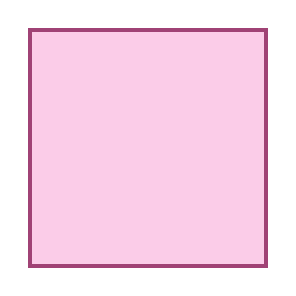
\begin{tikzpicture}
    \begin{scope}[thick,local bounding box=name]
    
         \ColorCells{       
            1/1/black!28/10,
            1/2/black!28/10,
            1/3/black!28/10,
            1/4/black!28/10,
            1/5/black!28/10,
            1/6/black!28/10,
            1/7/black!28/10,
            1/8/black!28/10,
            2/1/black!28/10,
            2/2/black!28/10,
            2/3/black!28/10,
            2/4/black!28/10,
            2/5/black!28/10,
            2/6/black!28/10,
            2/7/black!28/10,
            2/8/black!28/10,
            3/1/black!30/0,
            3/2/black!30/0,
            3/3/black!12/150,
            3/4/black!12/150,
            3/5/black!12/150,
            3/6/black!12/150,
            3/7/black!30/0,
            3/8/black!30/0,
            4/1/black!30/0,
            4/2/black!30/0,
            4/3/black!12/150,
            4/4/black!12/150,
            4/5/black!12/150,
            4/6/black!12/150,
            4/7/black!26/30,
            4/8/black!26/30,
            5/1/black!30/0,
            5/2/black!30/0,
            5/3/black!12/150,
            5/4/black!12/150,
            5/5/black!12/150,
            5/6/black!12/150,
            5/7/black!25/40,
            5/8/black!25/40,
            6/1/black!30/0,
            6/2/black!30/0,
            6/3/black!12/150,
            6/4/black!12/150,
            6/5/black!12/150,
            6/6/black!12/150,
            6/7/black!25/40,
            6/8/black!25/40,
            7/1/black!30/0,
            7/2/black!30/0,
            7/3/black!26/30,
            7/4/black!26/30,
            7/5/black!25/40,
            7/6/black!25/40,
            7/7/black!25/40,
            7/8/black!25/40,
            8/1/black!30/0,
            8/2/black!30/0,
            8/3/black!26/30,
            8/4/black!26/30,
            8/5/black!25/40,
            8/6/black!25/40,
            8/7/black!25/40,
            8/8/black!25/40
         }
    \draw [draw=magenta!60!black,fill=magenta, fill opacity=0.2,ultra thick](1,7) rectangle (4,4);
    \end{scope}
\end{tikzpicture}
} %%% case
    \caption{$I(x,y,t-1)$}
\end{figure}
 \columnbreak
 \begin{figure}[H]
    \centering
    \input{tikz/It2.tikz.tex}
    \caption{$I(x,y,t)$}
\end{figure}
\end{multicols}

\begin{multicols}{3}
 
  \begin{figure}[H]
    \centering
    \input{tikz/Ixdiff.tikz.tex}
    \caption{$I_y(x,y,t)$}
\end{figure}
 \columnbreak
 
  \begin{figure}[H]
    \centering
    \usetikzlibrary{calc}

\definecolor{DarkPink}{rgb}{0.55, 0.05, 0.37}

\newcommand*{\GridSize}{8}

\newcommand*{\ColorCells}[1]{% #1 = list of x/y/color
  \foreach \x/\y/\color/\text in {#1} {
    \node [fill=\color, draw=black, thick ,minimum size=1cm, line width=.8pt] 
      at (\x-.5,\GridSize+0.5-\y) [text=black] {\text};
    }%
}%

\tikzset{near start abs/.style={xshift=1cm}}
%%%%%


%\listfiles
\scalebox{0.42}{ %%% scale it
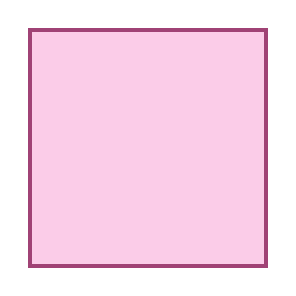
\begin{tikzpicture}
    \begin{scope}[thick,local bounding box=name]
    
         \ColorCells{
            1/1/black!30/?,
            1/2/black!30/?,
            1/3/black!30/?,
            1/4/black!30/?,
            1/5/black!30/?,
            1/6/black!30/?,
            1/7/black!30/?,
            1/8/black!30/?,
            2/1/black!30/0,
            2/2/black!13/140,
            2/3/black!13/140,
            2/4/black!13/140,
            2/5/black!13/140,
            2/6/black!28/-10,
            2/7/black!28/-10,
            2/8/black!30/0,
            3/1/black!30/0,
            3/2/black!30/0,
            3/3/black!30/0,
            3/4/black!30/0,
            3/5/black!30/0,
            3/6/black!27/20,
            3/7/black!27/20,
            3/8/black!30/0,
            4/1/black!30/0,
            4/2/black!30/0,
            4/3/black!30/0,
            4/4/black!30/0,
            4/5/black!30/0,
            4/6/black!25/40,
            4/7/black!25/40,
            4/8/black!30/0,
            5/1/black!30/0,
            5/2/black!12/-150,
            5/3/black!15/-120,
            5/4/black!15/-120,
            5/5/black!17/-110,
            5/6/black!28/10,
            5/7/black!28/10,
            5/8/black!30/0,
            6/1/black!30/0,
            6/2/black!12/-150,
            6/3/black!15/-120,
            6/4/black!15/-120,
            6/5/black!17/-110,
            6/6/black!30/0,
            6/7/black!30/0,
            6/8/black!30/0,
            7/1/black!30/0,
            7/2/black!30/0,
            7/3/black!30/0,
            7/4/black!30/0,
            7/5/black!30/0,
            7/6/black!30/0,
            7/7/black!30/0,
            7/8/black!30/0,
            8/1/black!30/?,
            8/2/black!30/?,
            8/3/black!30/?,
            8/4/black!30/?,
            8/5/black!30/?,
            8/6/black!30/?,
            8/7/black!30/?,
            8/8/black!30/?
         }
   \draw [draw=magenta!60!black,fill=magenta, fill opacity=0.2,ultra thick](1,7) rectangle (4,4);
    \end{scope}
\end{tikzpicture}
} %%% case
    \caption{$I_x(x,y,t)$}
\end{figure}
 \columnbreak
 
  \begin{figure}[H]
    \centering
    \usetikzlibrary{calc}

\definecolor{DarkPink}{rgb}{0.55, 0.05, 0.37}

\newcommand*{\GridSize}{8}

\newcommand*{\ColorCells}[1]{% #1 = list of x/y/color
  \foreach \x/\y/\color/\text in {#1} {
    \node [fill=\color, draw=black, thick ,minimum size=1cm, line width=.8pt] 
      at (\x-.5,\GridSize+0.5-\y) [text=black] {\text};
    }%
}%

\tikzset{near start abs/.style={xshift=1cm}}
%%%%%


%\listfiles
\scalebox{0.42}{ %%% scale it
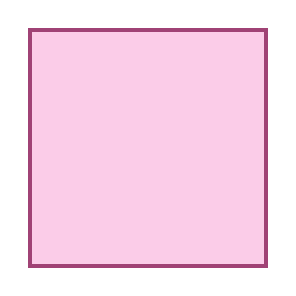
\begin{tikzpicture}
    \begin{scope}[thick,local bounding box=name]
    
         \ColorCells{
            %1/1/\color{rgb}
            1/1/black!30/0,
            1/2/black!30/0,
            1/3/black!30/0,
            1/4/black!30/0,
            1/5/black!30/0,
            1/6/black!30/0,
            1/7/black!30/0,
            1/8/black!30/0,
            2/1/black!30/0,
            2/2/black!13/140,
            2/3/black!13/140,
            2/4/black!13/140,
            2/5/black!13/140,
            2/6/black!30/0,
            2/7/black!30/0,
            2/8/black!30/0,
            3/1/black!30/0,
            3/2/black!12/150,
            3/3/black!30/0,
            3/4/black!30/0,
            3/5/black!30/0,
            3/6/black!12/-150,
            3/7/black!30/0,
            3/8/black!30/0,
            4/1/black!30/0,
            4/2/black!12/150,
            4/3/black!30/0,
            4/4/black!30/0,
            4/5/black!30/0,
            4/6/black!15/-120,
            4/7/black!30/0,
            4/8/black!30/0,
            5/1/black!30/0,
            5/2/black!12/150,
            5/3/black!30/0,
            5/4/black!30/0,
            5/5/black!30/0,
            5/6/black!17/-110,
            5/7/black!30/0,
            5/8/black!30/0,
            6/1/black!30/0,
            6/2/black!30/0,
            6/3/black!15/-120,
            6/4/black!15/-120,
            6/5/black!17/-110,
            6/6/black!17/-110,
            6/7/black!30/0,
            6/8/black!30/0,
            7/1/black!30/0,
            7/2/black!30/0,
            7/3/black!30/0,
            7/4/black!30/0,
            7/5/black!30/0,
            7/6/black!30/0,
            7/7/black!30/0,
            7/8/black!30/0,
            8/1/black!30/0,
            8/2/black!30/0,
            8/3/black!30/0,
            8/4/black!30/0,
            8/5/black!30/0,
            8/6/black!30/0,
            8/7/black!30/0,
            8/8/black!30/0
         }

    \end{scope}
    \draw [draw=magenta!60!black,fill=magenta, fill opacity=0.2,ultra thick](1,7) rectangle (4,4);
\end{tikzpicture}
} %%% case
    \caption{$I(x,y,t) - I(x,y,t-1)$}
\end{figure}
\end{multicols}
For example, given the sequence $I(x,y,t-1)$ \footnote{Image values, such as $I_x$ are tyipically represented by an 8-bit integer (\mintinline{latex}{uint8}). In this case we allow them to be negative without attempting to convert to the $[0,255]$ range for simplicity.} and $I(x,y,t)$ in the figures below, for the top left pixel in under the aperture we'd have the optical flow equation:
\begin{gather*}
I_x(1,1,t)u + I_y(1,1,t)v + I_t(1,1)= 0 \Rightarrow \\
100u + 100v + 140 = 0
\end{gather*}

\eqref{eq:opt_flow_unknowns} is called \emphasis{optical flow constraint equation} and there are a few more things it can tell us.

In \eqref{eq:opt_flow_unknowns}, we have \textit{two unknowns and one equation}. The equations also tells that the component of optical flow perpendicular to the image gradient (parallel to the edge) cannot be measured. Indeed, if $(u,v)$ satisfies it and $(u\prime,v\prime)$ is parallel to the edge, therefore $\nabla I \cdot \begin{bmatrix}u\prime & v\prime \end{bmatrix} = 0$, then also $\nabla I \cdot \begin{bmatrix}u+u\prime & v+v\prime \end{bmatrix}^T + I_t = 0$. Therefore \textit{only the component of optical flow perpendicular to the edge can be determined}.
\begin{multicols}{2}
 \columnbreak
\end{multicols}
\begin{figure}[H]
    \centering
    \includegraphics[height=3.0cm]{img/opt_flow/opt_flow_edge.PNG}
    \caption{Implication of brighness constraint equation -- optical flow along edge.}
    %\label{fig:my_label}
\end{figure}

From another point of view, \eqref{eq:opt_flow_unknowns}  is rewritten as
\begin{equation}
    v = -\frac{I_x}{I_y}u - \frac{I_t}{I_y}
\end{equation}
tells that optical flow given just the brightness constraint lies anywhere in a straight line in the $(u,v)$ space as illustrated below.
\begin{figure}[H]
    \centering
    \includegraphics[height=4.75cm]{img/opt_flow/opt_flow_straight_line.png}
    \caption{Caption}
    \label{fig:my_label}
\end{figure}
Suppose we have an optical flow that lies on the tip of $\boldsymbol{\rho}$ vector. Then if we decompose it in two vectors -- one normal to the line ($textbf{d}$) and one parallel ($\textbf{p}$), we have that the normal vector also points to the same optical flow lines. $d$ can be computed by the formula
\begin{equation}
    d =\frac{I_t}{\sqrt{I_x^2 + I_y^2}}
\end{equation}
In general, all vectors $(u,v)$ that line in the same optical flow line  can be decomposed as $d+p\prime$, where $p\prime$ is different and they have the same \emphasis{normal flow}.
\begin{corollary}
Only the \emphasis{normal flow} component $\textbf{d}$ of the optical flow can be estimated given the brightness constancy constraint.
\label{cor:opt_flow_line}
\end{corollary}
\begin{exmp}
% ref http://www.cs.umd.edu/~djacobs/CMSC426/OpticalFlow.pdf
Suppose we look through a $3\times3$ apperture at the following part of an image: 
\[
I(x,y,t) = \begin{bmatrix}1 & 1 & 1\\ 2 & 2 & 2\\3 & 3 &3 \end{bmatrix}
\]
Suppose that the optical flow is $(u,v)=(1,1)$. Therefore from the brighness constancy constraint for the new image $I(x,y,t+1)$ we have $I(x+1,y+1,t+1) = I(x,y,t+1)\Rightarrow I(x+1,y+1,t+1) = \begin{bmatrix} ? & ? & ?\\ 1 & 1 & 1\\ 2 & 2 & 2\end{bmatrix}$. Find (again, assuming it's not known) the optical flow from \eqref{eq:brightness_const} given images $I(x,y,t)$ and $I(x,y,t+1)$.
\end{exmp}
\begin{soln}
We will try to estimate it only for one pixel as the rest are similar, e.g. for the pixel at $(3,3)$:
\[
I(3,3,t) = 3, \; I(3,3,t+1) = 2 \Rightarrow I_t(3,3) = -1
\]
Also (assuming the $I_x(x,y) := I(x,y) - I(x-1,y)$ def/n for the discrete derivative), 
\[
I_x(3,3) = 3-3=0, \quad I_y(3,3) = 3-2=1
\]
So from the constraint equation:
\[
I_xu + I_yv + I_t = 0 \Rightarrow 0 + v = 1
\]
Therefore only one component of the optical flow can be estimated.
\end{soln}


The next sections describe how we can precisely determine the optical flow by introducing additional constraints.



\subsubsection{(Optional) The aperture problem and barber's pole illusion}


% see https://books.google.de/books?id=ZpnJDgAAQBAJ&pg=PA557&lpg=PA557&dq=barbers+pole+aperture+component+parallel+to+edge&source=bl&ots=XgKx1BiKtJ&sig=ACfU3U3gvGQWhn67_awTmuzuhMavV87Kxw&hl=en&sa=X&ved=2ahUKEwjZwIG3_7jiAhXGxqQKHQZACegQ6AEwC3oECAgQAQ#v=onepage&q=barbers%20pole%20aperture%20component%20parallel%20to%20edge&f=true
Imagine observing a group of straight lines translating vertically through a small aperture (Fig. \ref{fig:line_motion}). Imagine the same group of lines moving horizontally as shown in the same figure.. In both cases, the perceived motion is diagonally, particularly perpendicularly to the line orientation. That happens to be the intensity gradient too, as predicted by Corollary \ref{cor:opt_flow_line}. Because the line ends extend beyond the field of view, the actual direction of motion cannot be determined. In Fig. \ref{fig:line_motion}, although the line moves differently in each case, the eye is tricked into detecting the same motion perpendicular to the orientation.
\begin{figure}[H]
    \centering
    \includegraphics[height=6cm]{img/opt_flow/lines_motion.png}
    \caption{(a) A straight line translating vertically at three time points. The line ends extend beyond the receptive field. The component of motion parallel to the line's orientation cannot be detected. (b) Only the component of motion perpendicular to the line orientation can be detected. (c) A line translating horizontally through the blue receptive field. (d) Because its ends are not visible, only the component of motion perpendicular to its orientation can be detected.}
    \label{fig:line_motion}
\end{figure}
When looking at a barber pole, although it spins around the $z$ axis, therefore its stripes translate horizontally, it gives the perception that they move vertically. However, we saw that looking at a small part of the stripes through an aperture, they seem to move perpendicularly to their orientation -- not necessarily vertically. We will see that the key contributor to the apparent motion is the \textit{shape of the cylinder}. 

Imagine we are looking at a cylinder stripe through three apertures -- one at each edge and one on a central stripe (Fig \ref{fig:barbers_pole} (b)). Then the two apertures at the edge resolve the ambiguity due to their motion relative to the edge. Combining all three sensors together, we get an upwards motion.

\begin{figure}[H]
    \centering
    \includegraphics[height=5.5cm]{img/opt_flow/barbers_pole.png}
    \caption{The barber pole illusion. (a) It rotates about a central axis, however the observers perceive a vertical motion. (b) The visible endpoints at the edge apertures appear translate vertically (black arrows). For the central aperture, because of the aperture problem, its motion is ambiguous (grey arrows), as only the component perpendicular to the orientation can be determined. The visual system relies on the unambiguous vertical motion of the line endings. (d) The shape of the pole (or aperture) determines the direction in which the stripes appear to translate. If a rectangular window is oriented horizontally, then the stripes will appear to translate horizontally because most of the visible endpoints appear to translate this way. If the stripes translate behind  square aperture, then the conflicting motions of the endpoints will be superimposed to the direction perpendicular to the line, which will give the illusion of diagonal motion, just like in case of a circular aperture.}
    \label{fig:barbers_pole}
\end{figure}
Therefore the solution to unambiguous tracking is to track multiple ``good'' features together.




\subsection{Lucas-Kanade method}

% ref https://pdfs.semanticscholar.org/eec7/4fa786195ed9a8c754c989aa6b6eabf86ecd.pdf
They key assumption behind Lucas-Kanade is \emphasis{spatial coherence}. Spatial coherence is the assumption that \textit{nearby pixels will move together}, typically because they are part of the same object.

The spatial coherence constraint is applied to a pixel using a window of size $k\times k$. The assumption is that the neighbouring pixels in this window will have the same $(u,v)$. For example, in a $5\times5$ window and for each point $\textbf{p}_i$ in it (assuming greyscale input image), \eqref{eq:vec_grad_vec} applies 25 times:

\begin{gather}
I_t\left(\textbf{p}_i\right) + \nabla I\left(\textbf{p}_i\right)\begin{bmatrix}
 u & v\end{bmatrix} = 0 \Rightarrow \\
\underbrace{ \begin{bmatrix} 
 I_x\left(\textbf{p}_1 \right) & I_y\left(\textbf{p}_1 \right) \\
 I_x\left(\textbf{p}_2 \right) & I_y\left(\textbf{p}_2 \right) \\
 \vdots & \vdots \\
 I_x\left(\textbf{p}_{k\times k} \right) & I_y\left(\textbf{p}_{k\times k} \right)
 \end{bmatrix} }
 _{\bA}
 \begin{bmatrix}
 u \\ v
 \end{bmatrix} = 
 \underbrace{- \begin{bmatrix}
 I_t\left(\textbf{p}_1 \right)\\
 I_t\left(\textbf{p}_2 \right) \\
 \vdots \\
 I_t\left(\textbf{p}_{k \times k} \right)
 \end{bmatrix}}
 _{\textbf{b}}
\end{gather}
This produces an overly-constrained system of linear equations of the form $\textbf{Ad} = \textbf{b}$, i.e. we want to find a solution that minimises $\norm{\textbf{Ad} -\textbf{b}}^2$. it can be proven that the system can be rewrtitten
\[
(\textbf{A}^T\textbf{A})\textbf{d} = \textbf{A}^T\textbf{b}
\]
, where
\begin{equation}
    \textbf{A}^T\textbf{A} = 
    \begin{bmatrix}
        \sum\limits_{i=1}^{i=k^2}I_x\left(\textbf{p}_i\right)I_x\left(\textbf{p}_i\right) & \sum\limits_{i=1}^{i=k^2}I_x\left(\textbf{p}_i\right)I_y\left(\textbf{p}_i\right) \\
        \sum\limits_{i=1}^{i=k^2}I_y\left(\textbf{p}_i\right)I_x\left(\textbf{p}_i\right) & \sum\limits_{i=1}^{i=k^2}I_y\left(\textbf{p}_i\right)I_y\left(\textbf{p}_i\right)
    \end{bmatrix}, \quad
    \textbf{A}^T\textbf{b} = -
    \begin{bmatrix}
    \sum\limits_{i=1}^{i=k^2}I_x\left(\textbf{p}_i\right)I_t\left(\textbf{p}_i\right)   \\ 
    \sum\limits_{i=1}^{i=k^2}I_y\left(\textbf{p}_i\right)I_t\left(\textbf{p}_i\right) 
    \end{bmatrix}
\end{equation}
Finally, provided the invertability,  the solution  is:
\begin{equation}
    \textbf{d} := \begin{bmatrix}
    u & v
    \end{bmatrix}^T =  (\textbf{A}^T\textbf{A})^{-1}\textbf{A}^T\textbf{b}
    \label{eq:harris_lin_sq_sol}
\end{equation}
For the system to be solved, the following conditions must apply:
\begin{enumerate}
    \item $\textbf{A}^T\textbf{A}$ must be invertible.
    \item $\textbf{A}^T\textbf{A}$ should not be too small to cope with noise (i.e. the window patch for which $I_x, I_y$, hence $\textbf{A}$ is should have a strong texture). Mathematically, this implies that eigenvalues $\lambda_1, \lambda_2$ of $\textbf{A}^T\textbf{A}$ should not be too small \footnote{I have found that for windows of size approx. $13\times 13$ ``not too small'' means $\mathcal{O}(10^3)$ -- at least a few thousands.}.
	\item $\textbf{A}^T\textbf{A}$ should be well-conditioned, i.e. the condition number \footnote{For an explanation and derivation of the condition number, see \ref{app:cond_number}.} of $\bA$ $\kappa(\bA) = \lambda_1 / \lambda_2$ should not be too large ($\lambda_1$ is the larger eigenvalue). A good rule of thumb for ``too large'' is at the $10^3$ to $10^6$ scale.
\end{enumerate}
Under these conditions, there is no aperture problem and $\textbf{A}^T\textbf{A}$ is solvable. An interesting fact that relates $\bA^T\bA$ to the input image is that it can be written as:
\begin{gather}
    \textbf{A}^T\textbf{A} = 
    \begin{bmatrix}
    \sum I_x I_x & \sum I_xI_y \\
    \sum I_y I_x & \sum I_y I_y
    \end{bmatrix} = 
    \sum \begin{bmatrix}
    I_x \\ I_y
    \end{bmatrix}
    \begin{bmatrix}
    I_x & I_y
    \end{bmatrix} = 
    \sum \nabla I (\nabla I)^T
\end{gather}
, where $\sum \nabla I (\nabla I)^T$ is the dot product over the window. Matrix $\bA^T\bA$ is a \textit{Hessian matrix} (in discrete form) therefore is symmetric. Particularly, it's a \textit{Harris corner detector} matrix, which is used to detect features.

Now consider a corner or edge pixel $\textbf{p}_i$ at the centre of the $k\times k$ small window. For the gradient $\begin{bmatrix}I_x I_y \end{bmatrix}$, because pixels along the corner/ edge have similar magnitudes given by $\sqrt{I_x^2 + I_y^2}$, we can write \footnote{$k$ is unrelated to $\kappa$, just unfortunate notation.}:
\[
\sum \nabla I (\nabla I)^T = \kappa \nabla I(\textbf{p}_i) \left(\nabla I(\textbf{p}_i)\right)^T  = \kappa \norm{\nabla I(\textbf{p}_i)}^2
\]
Therefore:
\[
\underbrace{\left( \sum \nabla I (\nabla I)^T \right)}_{\bA^T\bA} \nabla I(\textbf{p}_i) = \kappa \norm{\nabla I(\textbf{p}_i)}^2 \nabla I(p_i)
\]
, where the sum is all over the window. The last equations tells us that the gradient vector $\nabla I(\textbf{p}_i)$ is an eigenvector of $\bA^T\bA$ with eigenvalue a multiple of $ \norm{\nabla I(p_i)}^2$. $\nabla I(\textbf{p}_i)$ points to the edge/ corner direction.

The second eigenvector of $\bA^T\bA$ is the vector $\textbf{u}_2$ is perpendicular to the first, i.e. perpendicular to the edge/ corner direction as Harris matrix is symmetric. 

\begin{corollary}
    For the Harris matrix $\bA^T\bA$ in Lucas Kanade method, its eigenvectors and eigenvalues of  relate to edge direction and magnitude. The eigenvector associated with the larger eigenvalue points in the direction of fastest intensity change.  The other eigenvector is orthogonal to it. If the matrix window overlaps a corner, both eigenvalues are large.
\end{corollary}
If $\lambda_1 \geq \lambda_2 > 0$ are the eigenvalues of $\bA^T\bA$ and $v_1,v_2$ their unit eigenvectors, and window $W$ sees and edge, then $v_1$ points perpendicularly to the edge. If window $W$ overlaps a corner, then $v_2$ points to the tip of the corner and $v_1$ is perpendicular to it. Mathematical derivation and interpretation of this conclusion is provided in \ref{app:harris_eigenvalues}.

The following graph summarises the relation of the eigenvalues of $\textbf{A}^T\textbf{A}$ to the nature of the image patch.

\begin{figure}[H]
    \centering
    \includegraphics[height=9cm]{img/opt_flow/harris_detector_eigen.jpg}
    \caption{What the eigenvalues $M = \textbf{A}^T\textbf{A}$ mean regarding the region under the $k\times k$ window.}
\end{figure}
\begin{exmp}
Assume that we see the image patches
\[
I = 
\begin{bmatrix}
0 & 0 & 0 & 10 & 10 \\
0 & 0 & 0 & 10 & 10\\
0 & 0 & 0& 20 & 10 \\
10 & 10 & 10 & 20 & 10 \\
10 & 10 & 10 & 10 & 10 \\
\end{bmatrix}, \quad
J =
\begin{bmatrix}
0 & 0 & 0 & 20 & 20 \\
0 & 0 & 0 & 30 & 20 \\
0 & 0 & 0 & 40 & 20 \\
0 & 0 & 0 & 20 & 20 \\
0 & 0 & 0 & 20 & 20 \\
\end{bmatrix}
\]
at two different locations when scanning with a $5\times 5$ window. Determine which one is edge and which a corner using the Hessian matrix. When computing the discrete derivatives, extrapolate the pixels around and off the image to the nearest border pixel.
\end{exmp}
Begin with $I$ and compute its partial derivatives \footnote{In the code, partial derivatives are computed by convolution. Convolution of an image $I$ with a kernel $K$, e.g. $K=\begin{bmatrix}
-1 & 0 & 1 \end{bmatrix}$ and by replicating border pixels is implemented in OpenCV by \mintinline{python}{cv2.filter2D(I, -1, [1 0 -1], borderType=cv2.BORDER_REPLICATE)}. Care needs to be taken when selecting the type of $I$ (unsigned/ signed) int, as the output type is the same.}.
\[
I_x = 
\begin{bmatrix}
0 & 0 & 10 & 10 & 0 \\
0 & 0 & 10 & 10 & 0\\
0 & 0 & 20& 10 & 0 \\
0 & 0 & 10 & 0 & -10 \\
0 & 0 & 0 & 0 & 0
\end{bmatrix}, \quad
I_y = 
\begin{bmatrix}
0 & 0 & 0 & 10 & 0 \\
0 & 0 & 0 & 10 & 0\\
10 & 10 & 10 & 20 & 0 \\
10 & 10 & 10 & -10 & 0 \\
0 & 0 & 0 & -10 & 0 
\end{bmatrix}, \quad
I_x *. I_y  = 
\begin{bmatrix}
0 & 0 & 0 & 100 & 0 \\
0 & 0 & 0 & 100 & 0\\
0 & 0 & 200 & 200 & 0 \\
0 & 0 & 100 & 0 & 0 \\
0 & 0 & 0 & 0 & 0 
\end{bmatrix}
\]
, where $*.$ denotes the element-wise product. Therefore the Hessian (correlation) matrix is:
\[
M = \begin{bmatrix}
\sum I_x^2 & \sum I_xI_y \\
\sum I_yI_x & \sum I_y^2
\end{bmatrix} =
\begin{bmatrix}
1100 & 700 \\
700 & 1400
\end{bmatrix}
\]
The eigenvalue and unit eigenvector matrix of $M$ are\footnote{In Numpy, eigendata are computed as: \mintinline{python}{w, v = np.linalg.eig(M)}.}
\[
\Lambda = 
\begin{bmatrix}
1965.89 & \\
 & 534.10
\end{bmatrix},\quad 
V =
\begin{bmatrix}
0.628 & -0.777\\
0.777 & 0.628
\end{bmatrix}
\]
$v_1 = \begin{bmatrix} 0.628 & 0.777 \end{bmatrix}^T$ forms an angle of $51.05\degree$, i.e. points perpendicularly to the direction of the corner tip, as expected.

For $J$ we have:
\[
J_x = 
\begin{bmatrix}
0 & 0 & 20 & 20 & 0 \\
0 & 0 & 30 & 20 & 0 \\
0 & 0 & 40 & 20 & 0 \\
0 & 0 & 20 & 20 & 0 \\
0 & 0 & 20 & 20 & 0 \\
\end{bmatrix},  \quad
J_y = 
\begin{bmatrix}
0 & 0 & 0 & 10 & 0 \\
0 & 0 & 0 & 20 & 0 \\
0 & 0 & 0 & -10 & 0 \\
0 & 0 & 0 & -20 & 0\\
0 & 0 & 0 & 0 & 0 
\end{bmatrix}, \quad
J_x *. J_y = 
\begin{bmatrix}
0 & 0 & 0 & 200 & 0 \\
0 & 0 & 0 & 100 & 0 \\
0 & 0 & 0 & -200 & 0 \\
0 & 0 & 0 & -100 & 0 \\
0 & 0 & 0 & 0 & 0 \\
\end{bmatrix}
\]
Therefore the correlation Hessian matrix is
\[
M = \begin{bmatrix}
\sum J_x^2 & \sum J_xJ_y \\
\sum J_yJ_x & \sum J_y^2
\end{bmatrix} =
\begin{bmatrix}
5700 & 0 \\
0 & 1000
\end{bmatrix}
\]
The eigendata are
\[
\Lambda = \begin{bmatrix}
5700 & \\
 & 1000
\end{bmatrix},\quad
V = 
\begin{bmatrix}
1 & 0 \\ 0 & 1
\end{bmatrix}
\]
The eigenvector $v_1 = \begin{bmatrix}1 & 0\end{bmatrix}$ corresponding to the largest eigenvalue points to the fastest change, i.e. perpendicularly to the vertical edge.


\subsubsection{Implementation of Lucas-Kanade from scratch}

An implementation of Lucas-Kanade based on what has been established so far in this section has been written in Python from scratch and is listed in \ref{app:lucas_kanade_scratch}.

The script can be run as:
\begin{verbatim}
$ python lucas_kanade_scratch.py image_1_path image_2_path [min_eigenvalue_threshold]
\end{verbatim}
, where \mintinline{python}{min_eigenvalue_threshold} is an optional argument. The script writes the output result to directory \mintinline{python}{/tmp}. Tip: to exaggerate the optical flow result, change the following line
\begin{verbatim}
feature_pts.append(Feature((c,r), tuple(vec_xy)))
\end{verbatim}
to, e.g.
\begin{verbatim}
feature_pts.append(Feature((c,r), tuple(5 * vec_xy)))
\end{verbatim}
The figure below shows the result of the algorithm from scratch for a sequence of cars moving on two lanes. The output vectors (greens) are slightly exaggerated.
\begin{figure}[H]
    \centering
    \includegraphics[height=5.5cm]{img/opt_flow/scratch_output.png}
    \caption{Lucas Kanade from scratch motion vectors. Window size is $13\times 13$, minimum corner ratio is $10^3$ and minimum eigenvalue threshold is $3\cdot 10^4$.}
    \label{fig:my_label}
\end{figure}

\begin{itemize}
    \item A \textit{weakness} of this algorithm is that the eigenvalue ratio is not always a good measure to select corners. As a result, a lot of false positive (FP) features are considered. A better measure is Harris's corner detector response function $R = \lambda_1\lambda_2 - k (\lambda_1 + \lambda_2)^2$, where $k$ is a constant. This will not be discussed in this tutorial.
    \item Another \textit{weakness} is that is only considers small feature motions. An improvement is to use the the hierarchical Lucas Kanade, which uses image pyramids (downsampled of the original), and operates from the smallest image to the largest, given previous knowledge. Hierarchical Lucas Kanade will be discussed later.
\end{itemize}


\subsubsection{Implementation of Lucas-Kanade with OpenCV}

In OpenCV, Lucas-Kanade tracks ``features'' (essentially corners) using the \mintinline{python}{cv2.goodFeaturesToTrack()} method. This returns an array of potentially good points that Lucas-Kanade would like to track. It is followed by \mintinline{python}{cv2.calcOpticalFlowPyrLK()}, which takes in the two image frames and the candidate points and returns their new positions, as well as which points are valid from one frame to another. The calls are described in detail below.

\begin{minted}{python}
cv2.goodFeaturesToTrack(image, maxCorners, qualityLevel, minDistance[, corners[, mask[, blockSize
[, useHarrisDetector[, k]]]]]) -> corners
\end{minted}
\begin{itemize}
    \item \mintinline{python}{image}:  Input 8-bit (\mintinline{python}{np.uint8}) or floating-point 32-bit, single-channel image, e.g. a greyscale one.
    \item \mintinline{python}{maxCorners}: Maximum number of corners to return. If there are more corners than are found, the strongest of them is returned.
    \item \mintinline{python}{qualityLevel}: Quality level threshold as a fraction of the corner with best quality for qwhich corners to retain. For example, if the corner with best quality has a measure of 1500 and \mintinline{python}{qualityLevel = 0.1}, then only corners with measure of at least 150 are considered. 
    \item \mintinline{python}{minDistance}: Minimum possible Euclidean distance between the returned corners.
    \item \mintinline{python}{[mask]}: Optional region of interest. If the image is not empty (it needs to have the type \mintinline{python}{CV_8UC1} (essentially \mintinline{python}{np.uint8}) and the same size as image ), it specifies the region in which the corners are detected. If \mintinline{python}{mask[i, j] == 255}, then the pixel of the original image at \mintinline{python}{i, j} is considered, if \mintinline{python}{mask[i, j] == 0} it is ignored.
    \item \mintinline{python}{[blockSize]}: Size of an average block for computing a derivative covariation matrix over each pixel neighborhood. See \mintinline{python}{cornerEigenValsAndVecs()}. 
    \item \mintinline{python}{corners}: array of 2D ``good'' points in a column vector. It is of shape \mintinline{python}{(n, 1, 2)} -- same as the \mintinline{python}{prevPts} in the \mintinline{python}{cv2.calcOpticalFlowPyrLK()} call below,
\end{itemize}


\begin{minted}{python}
cv2.calcOpticalFlowPyrLK(prevImg, nextImg, prevPts[, nextPts[, status[, err[, winSize[,
maxLevel[, criteria[, flags[, minEigThreshold]]]]]]]]) -> nextPts, status, err
\end{minted}
\begin{itemize}
    \item \mintinline{python}{prevImg}: first 8-bit input image or pyramid constructed by \mintinline{python}{buildOpticalFlowPyramid}. 
    \item \mintinline{python}{nextIng}: second input image or pyramid of the same size and the same type as \mintinline{python}{prevImg}. 
    \item \mintinline{python}{prevPts}: vector of 2D points for which the flow needs to be found; point coordinates must be single-precision floating-point numbers. 
    \item \mintinline{python}{[nextPts]}: output vector of 2D points (with single-precision floating-point coordinates) containing the calculated new positions of input features in the second image; when \mintinline{python}{OPTFLOW_USE_INITIAL_FLOW} flag is passed, the vector must have the same size as in the input. 
    \item \mintinline{python}{[winSize]}: size of the search window at each pyramid level (tuple).
    \item \mintinline{python}{[maxLevel]}: 0-based maximal pyramid level number; if set to 0, pyramids are not used (single level), if set to 1, two levels are used, and so on; if pyramids are passed to input then algorithm will use as many levels as pyramids have but no more than maxLevel.
    \item \mintinline{python}{[criteria]}: termination criteria of the iterative search algorithm. Number of iterations and search window displacment need to be specified, e.g. as \mintinline{python}{cv2.TERM_CRITERIA_EPS | cv2.TERM_CRITERIA_COUNT, 10, 0.03))}. 
\end{itemize}
\textit{Tips}: \mintinline{python}{nextPts}, as returned by \mintinline{python}{calcOpticalFlowPyrLK} is a vector of 2D points, where each point is represented by an array \mintinline{python}{[x, y]}, therefore \mintinline{python}{nextPts} is of size \mintinline{python}{(n, 1, 2)}. To select the good points, we choose those whose status is 1 by  \mintinline{python}{good_new = good_new[st == 1]}. \mintinline{python}{good_new} is now of size \mintinline{python}{(n, 2)} therefore needs to be reshaped to \mintinline{python}{(n, 1, 2)} so it can be passed in the next round of Lucas-Kanade as the previous good points. The \mintinline{python}{calcOpticalFlowPyrLK} workflow, taken from OpenCV's tutorials \cite{docopencvoptflow}, is summarised as
\begin{minted}{python}
p1, st, err = cv2.calcOpticalFlowPyrLK(old_gray, frame_gray, p0, None, **lk_params)
good_new = p1[st==1]
# display the points etc.
p0 = good_new.reshape(-1,1,2)
# then loop again
\end{minted}
Note that this way of selecting new points tends to reduce their number. A class to configure and run Lucas-Kanade in OpenCV has been listed in \ref{app:lucas_kanade_opencv}.

\subsection{Hierarchical Lucas-Kanade}


%%%%%%%%%%%%%%%%%%%%
% see this: https://ags.cs.uni-kl.de/fileadmin/inf_ags/opt-ss14/OPT_SS2014_lec06.pdf
% eigenvalues and edges: https://dsp.stackexchange.com/questions/10104/why-eigenvalues-concerned-in-harris-corner-detection
% harris and image: https://en.wikipedia.org/wiki/Harris_Corner_Detector
%PCA : http://www.math.union.edu/~jaureguj/PCA.pdf
% corrected: https://courses.cs.washington.edu/courses/csep576/05wi/lectures/motion.pdf
% kinda helpful: http://cs.haifa.ac.il/hagit/courses/CV/Lectures/CV05_Motion_X4.pdf
% 2nd moment matrix: https://www.uio.no/studier/emner/matnat/its/nedlagte-emner/UNIK4690/v16/forelesninger/lecture_3_2_1_corner_features.pdf
%%%%%%%%%%%

% good: http://www.cs.cmu.edu/~16385/s17/Slides/15.1_Tracking__KLT.pdf
% harris matrix: http://www.cs.cornell.edu/courses/cs4670/2015sp/lectures/lec07_harris_web.pdf
% harris matrix more: https://ags.cs.uni-kl.de/fileadmin/inf_ags/opt-ss14/OPT_SS2014_lec02.pdf
% see http://www.cs.cmu.edu/~16385/s17/Slides/14.4_Alignment__LucasKanade.pdf
% https://pdfs.semanticscholar.org/eec7/4fa786195ed9a8c754c989aa6b6eabf86ecd.pdf
% https://ags.cs.uni-kl.de/fileadmin/inf_ags/opt-ss14/OPT_SS2014_lec06.pdf
% http://mccormickml.com/2013/03/30/ucf-lecture-6-optical-flow/
% really good: https://www.cse.iitb.ac.in/~ajitvr/CS763_Spring2017/OpticalFlow.pdf
% https://jayrambhia.com/blog/lucas-kanade-tracker
% http://www.cs.umd.edu/~djacobs/CMSC426/OpticalFlow.pdf
% http://web.yonsei.ac.kr/jksuhr/articles/Kanade-Lucas-Tomasi%20Tracker.pdf
% https://www.cc.gatech.edu/~afb/classes/CS4495-Fall2014/slides/CS4495-MotionModels.pdf
% https://ags.cs.uni-kl.de/fileadmin/inf_ags/opt-ss14/OPT_SS2014_lec06.pdf
% https://files.ifi.uzh.ch/rpg/teaching/2015/11_tracking.pdf
% good http://www.cs.princeton.edu/courses/archive/fall11/cos429/notes/cos429_f11_lecture08_motion.pdf
% warp: https://www.cc.gatech.edu/~afb/classes/CS4495-Fall2014/ProblemSets/PS5/burt-trcom1983.pdf
% warp: http://www.ece.tufts.edu/en/74/10_warping.pdf

% derivation: 
% http://campar.in.tum.de/twiki/pub/Chair/TeachingWs12TDCV/template_tracking.pdf
% https://www.ri.cmu.edu/pub_files/pub3/baker_simon_2004_1/baker_simon_2004_1.pdf

% harris: https://books.google.de/books?id=MgIVyAWf9VUC&pg=PA110&lpg=PA110&dq=how+do+eigenvectors+relate+to+edge+direction&source=bl&ots=go7hhKCyWT&sig=ACfU3U0nDgKMcvMa7b03YINuLJkzKcINKQ&hl=en&sa=X&ved=2ahUKEwinw6LY0bnjAhWHRMAKHejCA044FBDoATAFegQIBxAB#v=onepage&q=how%20do%20eigenvectors%20relate%20to%20edge%20direction&f=false




%%%%%%%%%%%%%%%%%%%%%%%%%%%%%%%%%%%%%%%%%%%%%%%%%%%%%%%%%%%%%%%%%%%%%%%%%%%%%%%%%%%%%%%%%%%%%%%%%%%%
% APPENDICES
%%%%%%%%%%%%%%%%%%%%%%%%%%%%%%%%%%%%%%%%%%%%%%%%%%%%%%%%%%%%%%%%%%%%%%%%%%%%%%%%%%%%%%%%%%%%%%%%%%%%
\newpage
\appendix

\section{Appendices}

% ------------------------ New appendix ------------------------ %
\newpage
\subsection{HSV domain}
\label{app:hsv_domain}

\TODO[why is HSV colour scheme used in tracking/ detection?]





% ------------------------ New appendix ------------------------ %
\newpage


\subsection{Histogram backprojection implementation from scratch -- source code}
\label{app:hist_backproj_src}
\lstinputlisting[language=python,caption={Histogram backprjection from scratch (\detokenize{src/hist_backproj/backproj.py)}.}, label=src:mylabel]{src/hist_backproj/backproj.py}



% ------------------------ New appendix ------------------------ %
\newpage
\subsection{Histogram backprojection implementation using OpenCV - source code}
\label{app:hist_backproj_src_opencv}
\lstinputlisting[language=python,caption={Histogram backprjection using OpenCV's \mintinline{python}{calcBackProject} (\detokenize{src/hist_backproj/backproj_cv.py)}.}]{src/hist_backproj/backproj_cv.py}
%\inputminted{python}{src/hist_backproj/backproj_cv.py}


% ------------------------ New appendix ------------------------ %
\newpage
\subsection{My mean shift implementation from scratch -- source code}
\label{app:mean_shift_mine}
\lstinputlisting[language=python,caption={Mean shift using OpenCV's \mintinline{python}{meanShift} (\detokenize{src/mean_shift/my_mean_shift.py)}.}]{src/mean_shift/my_mean_shift.py}
%\inputminted{python}{src/hist_backproj/backproj_cv.py}


% ------------------------ New appendix ------------------------ %
\newpage
\subsection{Mean Shift implementation using OpenCV - source code}
\label{app:mean_shift_opencv}
\lstinputlisting[language=python,caption={Mean shift using OpenCV's \mintinline{python}{meanShift} (\detokenize{src/mean_shift/mean_shift_cv.py)}.}]{src/mean_shift/mean_shift_cv.py}
%\inputminted{python}{src/hist_backproj/backproj_cv.py}


% ------------------------ New appendix ------------------------ %
\newpage
\subsection{Condition number of a matrix}
\label{app:cond_number}

In short, the condition number of a matrix measures how it can be inverted
\subsubsection{Normal matrix}
Below are the definition and a basic property just for completeness.
\begin{definition}
	A square matrix $\bA$ is \emphasis{normal} when
	\begin{equation}
		\bA^H\bA - \bA\bA^H = 0
	\end{equation}
	, where $H$ is the Hermitian, i.e. conjugate transpose operator.
\end{definition}
A matrix $\bA$ can be normal without being Hermitian, i.e. the $M = \begin{bmatrix}5 & 0\\0 & 2-3i \end{bmatrix}$. Normal matrices are unitarily diagonalisable, i.e. if $\bA$ is normal there exists a unitary matrix such the:
\begin{equation*}
	D = U A U^T	
\end{equation*}
is diagonal.
\begin{theorem}
	A matrix is normal iff it is unitarily diagonalisable.
\end{theorem}
\begin{proof}
	($\Leftarrow$)

	If $\bA$ is unitarily dia/ble, then:
	\begin{gather*}
		\bA = U \Lambda U^H	\\
		\therefore \bA\bA^H = U \Lambda U^H U \Lambda^H U^H = U \Lambda^2 U^H, \\
		\bA^H \bA = U \Lambda^H U^H U \Lambda U^H = U \Lambda^2 U^H
	\end{gather*}

	($\Rightarrow$)
	
	\textit{Hint:} Write $A$ as the sum of its real and imaginary part, i.e. $\bA = \bB + i\bC$. Full proof is omitted.
\end{proof}


\subsubsection{The spectral matrix norm}


\begin{definition}[matrix norm]
The matrix norm, denoted as $\norm{\:.\:}$, is a function $\setR^{m \times n}\rightarrow \setR$ that satisfies all of the following properties:
\begin{enumerate}
    \item $\norm{A} \geq 0$ if $\textbf{A} \neq \textbf{0}_{m \times  n}$ -- positive valued
    \item $\norm{A} = 0$ iff $\textbf{A}=\textbf{0}_{m\times n}$ -- definite
    \item $\norm{\alpha \textbf{A}} = \left| \alpha \right|\norm{A}$ for every $\alpha \in \setR$ -- homogeneous
    \item $\norm{\textbf{A}-\textbf{B}} \leq \norm{\textbf{A}} + \norm{\textbf{B}}$ for every $\textbf{A}, \textbf{B} \in \setR^{m \times n}$ -- triangular inequality
\end{enumerate}
\end{definition}
% properites proof: https://www.math.uh.edu/~jingqiu/math4364/iterative_linear_system.pdf
It can be shown that the spectral norm defined below satisfies these properties \cite{lecnormsproof}, \cite{lecconrad} \footnote{Another proof by SVD here \cite{lecdalhe}.}. Note that $\norm{\textbf{x}}_2$ is simply the vector norm of $\textbf{x}\in \setR^n$, which can be defined as:
\begin{equation}
\norm{\textbf{x}}_2 = (\textbf{x}^T\textbf{x})^{\frac{1}{2}} = \left(\sum\limits_{i=0}^{n}x_i^2\right)^{\frac{1}{2}}     
\end{equation}
\begin{definition}[spectral norm of matrix]
The \emphasis{spectral} (or $\ell_2$, or induced matrix) norm of a matrix $\textbf{A}\in \setR^{m\times n}$ is defined as:
\begin{equation}
    \norm{\textbf{A}}_2 = \underset{\norm{\textbf{x}}_2=1}{\max}\norm{\textbf{Ax}}_2 
\end{equation}
Although we'll use the former, an equivalent defintion is
\begin{equation}
    \norm{\textbf{A}}_2 = \underset{\substack{\textbf{x}\in\setR^n \\ \textbf{x} \neq 0}}
    {\max} 
    \frac{{\max}\norm{\textbf{Ax}}_2}{\norm{\textbf{x}}_2}
\end{equation}
\end{definition}

We often define the spectral norm via the following alternative expression.
\begin{lemma}[spectral norm equal largest singular value]
Given a matrix $\textbf{A}_{m\times n}$ and a unit vector $\textbf{x} \in \setR^n, \; \norm{\textbf{x}}=1$, the maximum value of the norm-2 of $\textbf{A}$ is $\sqrt{\lambda_{1}(\textbf{A}^T\textbf{A})}$, where  $\lambda_{1}(\textbf{A}^T\textbf{A})$ is the largest eigenvalue of $\textbf{A}^T\textbf{A}$. 
\begin{equation}
    \underset{\norm{\textbf{x}}_2=1}{max}\norm{\textbf{Ax}}_2 = \sqrt{\lambda_{1}(\textbf{A}^T\textbf{A})}
\end{equation}
\end{lemma}
\begin{proof}
\[
\norm{\textbf{Ax}}_2^2 = (\textbf{Ax})^T(\textbf{Ax})= \textbf{x}^T\textbf{A}^T\textbf{Ax}  \tag{1}
\]
Matrix $\textbf{A}^T\textbf{A}$ is symmetric therefore diagonalisable, hence we can factor it as:
\[
\textbf{A}^T\textbf{A} = \textbf{V}^T\boldsymbol{\Lambda}\textbf{V}   \tag{2}
\]
, where $\textbf{V}$ is an orthonormal matrix, so $\textbf{V}^T\textbf{V}= \textbf{I}$. $\boldsymbol{\Lambda}$ is a diagonal matrix of the non-negative eigenvalues of $\textbf{A}^T\textbf{A}$, i.e.
\[
\boldsymbol{\Lambda} =
\begin{bmatrix}
\lambda_1 & & \\
 & \ddots & \\
 & & \lambda_n
\end{bmatrix}
\]
As a convention, we write the eigenvalues in decreasing order, such that $\lambda_1\geq \ldots \geq \lambda_n \geq 0$. Given the diagonalisation in Eq. (2), we square of the norm becomes:
\[
\begin{split}
\textbf{x}^T\textbf{A}^T\textbf{Ax} = \textbf{x}^T\textbf{V}^T\boldsymbol{\Lambda}\underbrace{\textbf{Vx}}_{\textbf{y}}&=\textbf{y}^T\boldsymbol{\Lambda}\textbf{y} \\
& = \sum\limits_{i}\lambda_i y_i^2\\
& \stackrel{\lambda_1\geq \ldots \geq \lambda_n}{\leq} \lambda_1 \sum\limits_{i}y_i^2 \stackrel{\norm{y}_2=1}{=} \lambda_1
\end{split}
\]
The expansion to the first sum was done by using the theory for the \textit{quadratic form} of the product. We have proven the upper bound

\begin{gather*}
\norm{Ax}_2^2 = \textbf{x}^T\textbf{A}^T\textbf{Ax} \leq \lambda_1 \Rightarrow
\norm{Ax}_2 \leq \sqrt{\lambda_1}
\end{gather*}
, where $\lambda_1 = \lambda_1(\textbf{A}^T\textbf{A})$, also called a \emphasis{singular value} of $\textbf{A}$. We show that a maximum of $\norm{Ax}_2$ is attained at $\sqrt{\lambda_1}$ by setting $\textbf{x}=\textbf{u}_1$, where $\textbf{u}_1$ is the unit eigenvector corresponding to the maximum eigenvalue $\lambda_1$:
\[
\norm{Au_1}_2 = \norm{\lambda_1u_1}_2 = \left|\lambda_1 \right| = \lambda_1
\]
We have proven that
\[
\underset{\norm{\textbf{x}}_2=1}{max}\norm{\textbf{Ax}}_2 = \sqrt{\lambda_{1}(\textbf{A}^T\textbf{A})}
\]
\end{proof}
% interpr: http://www.seas.ucla.edu/~vandenbe/133A/lectures/condition.pdf



\subsubsection{The condition number of a matrix}

Suppose we want to compute $\by = \bA \bx$ but because of noise $\bA$ it perture by a small amount $\textbf{E}$ to $\bA + \textbf{E}$ so instead we compute $\hat{\by} = (\bA + \textbf{E})\bx$.Then the absolute error is
\begin{equation*}
	\norm{\by - \hat{\by}}= \norm{\textbf{Ex}}
\end{equation*}
The \textit{relative error}r of the output, which is what we want to measure, is:
\begin{equation}
	\frac{\norm{\by - \hat{\by}}}{\norm{\by}} = \frac{\norm{\textbf{Ex}}}{\norm{\by}} \tag{1}
\end{equation}
If we assume that $\bA$ is invertible, then by the dot product inequality for the norm in the numerator we have:
\begin{equation*}
	\norm{E \bx} = \norm{E \bA^{-1}y} \leq \norm{E} \norm{\bA^{-1}}\norm{\by}	
\end{equation*}
Therefore Eq. (1) yields the inequality:
\begin{equation*}
	\frac{\norm{\by - \hat{\by}}}{\norm{\by}}  \leq \norm{E}\norm{\bA^{-1}} = \norm{\bA}\norm{\bA^{-1}} \frac{\norm{E}}{\norm{\bA}} = \kappa(\bA)  \frac{\norm{E}}{\norm{\bA}} 
\end{equation*}
\begin{definition}
The scalar $\kappa(\bA) = \norm{\bA}\norm{\bA^{-1}}$ is called \emphasis{condition number} of matrix $\bA$.
\end{definition}
Therefore, when computing the relative error, the perturbation $E$ is multiplied by condition number $\kappa(\bA) = \norm{\bA}\norm{\bA^{-1}}$. The condition 
 characterizes the relationship between a small relative perturbation to $\bA$ and a small relative perturbation to the matrix-vector product $\bA\bx$. We say that a matrix $\bA$ in the linear system $\bA\bx = \by$ is \emphasis{ill-conditioned} when  its condition number is large.

Recall that $\norm{.}_2$ operator is defined as the maximum amount that matrix $\bA$ can stretch a unit vector by, i.e.:
\begin{equation*}
	M = \norm{\bA} = 	
    \frac{{\max}\norm{\textbf{Ax}}_2}{\norm{\textbf{x}}_2}
\end{equation*}
The norm of the inverse measures how much mapping $\bA$ can shrink unit vectors as:
\begin{equation*}
	% TODO: y= Ax
	m = \norm{\bA^{-1}} = \max\frac{\bA^{-1}\by}{\by} = \frac{1}{ \min\frac{\bA^{-1}\by}{\by}} = \min \frac{\by}{\bA^{-1}\by}=\min \frac{\bA \bx}{\bx} 
\end{equation*}
Therefore the condition number measures ratio of the maximum stretching over maximum shrinkage a matrix $\bA$ can apply to unit vectors. 

If a matrix is singular, then its condition number is infinite. A very large condition number implies a matrix is close to being singular.

\begin{corollary}
	If a matrix $\bA$ is invertible, then its condition number is given by:
	\begin{equation}
		\kappa(\bA) = \frac{\sqrt{\lambda_1(\bA^T\bA)}}{\sqrt{\lambda_n(\bA^T\bA)}}
	\end{equation}
, where $\lambda_1(\bA^T\bA)$ and $\lambda_n(\bA^T\bA)$ are the largest and smallest eigenvalues of $\bA^T\bA$.
\end{corollary}
\begin{proof}
	% TODO: where?
	It has already been derived that $\norm{\bA} = \lambda_1(\bA^T\bA)$. We also know for the singular values of the inverse that:
	\begin{equation*}
		\sigma_i(\bA) = 1 / \sigma_i(\bA^{-1})
	\end{equation*}
	Therefore for the maximum singular value of $\bA$, $\sigma_{\max}(\bA)$:
	\begin{equation*}
		\sigma_{\max}(\bA) = 1 / \sigma_{\min}(\bA^{-1})	
	\end{equation*}
	The condition number can then be written as:
	\begin{equation*}
		\kappa(\bA) = \norm{\bA} \norm{\bA^{-1}} = \frac{\sigma_{\max}(\bA)}{\sigma_{\min}(\bA)}	
	\end{equation*}
\end{proof}


\begin{corollary}
	If a matrix $\bA$ is invertible and normal, the condition number is given by:
	\begin{equation*}
		\kappa(\bA) = \frac{\left|\lambda_{\max}(\bA)\right|}{\left|\lambda_{\min}(\bA)\right|}	
	\end{equation*}
\end{corollary}
\begin{proof}
	$\bA$ being normal means it can be factorised as:
	\begin{equation*}
		% ref https://math.stackexchange.com/questions/2817630/why-the-condition-number-of-matrix-given-by-eigenvalues	
		\bA = U \Lambda U^T
	\end{equation*}
	, where $U$ is unitary (orthonormal) and $\Lambda$ is the diagonal matrix of eigenvalues of $\bA$. Therefore $\bA^TA = U \Lambda U^T U \Lambda U^T = U \Lambda^2 U^T$. For the singular values of $\bA$:
\begin{equation*}
	\sigma_{\max}(\bA) = \sqrt{\lambda_{\max}(\bA^T \bA)} = \sqrt{\lambda_	{\max}(U \Lambda^2 U^T)} = \sqrt{\lambda_{\max}(\bA)^2} = \left| \lambda_{\max} \right|
\end{equation*}
	Similarly, $\sigma_{\min}(\bA) = \left| \lambda_{\min}(\bA)\right|$. Finally,
	\begin{equation*}
		\kappa(\bA) = \frac{\left| \lambda_{\max}(\bA)\right|}{\left| \lambda_{\min}(\bA)\right|}		
	\end{equation*}
	Another, more concise proof, by SVD is given in \cite{stackratioproof}.
\end{proof}
% http://www.cs.utexas.edu/users/flame/Notes/NotesOnConditioning.pdf
% https://people.sc.fsu.edu/~jburkardt/classes/gateway_2014/lecture_week04.pdf
% http://www.phys.uconn.edu/~rozman/Courses/m3511_18s/downloads/condnumber.pdf
% http://www.cs.cornell.edu/courses/cs3220/2009sp/notes/condition.pdf
% inp out http://fourier.eng.hmc.edu/e176/lectures/NM/node2.html
% http://www.cse.iitm.ac.in/~vplab/courses/LARP_2018/Matrix-Vector%20and%20Matrix%20Norms-3.pdf


% (extra) appls: https://www.tu-braunschweig.de/Medien-DB/iwr/lehre/lec2.pdf



% ------------------------ New appendix ------------------------ %
\newpage
\subsection{Eigenvalues of Harris matrix -- why do they indicate corners and edges?}
\label{app:harris_eigenvalues}

Lucas-Kanade method uses the matrix $M = \begin{bmatrix}    \sum I_x I_x & \sum I_xI_y \\
    \sum I_y I_x & \sum I_y I_y \end{bmatrix}$ to solve for the displacement of a ``feature'' from one frame to another. The matrix needs to be inverted as part of the least squares solution as shown in the main section of the document \eqref{eq:harris_lin_sq_sol}. But $\textbf{M}$ also tells us about the nature of the feature -- whether it's an edge, corner, or simply a flat area. \textit{But why}?

% ref http://faculty.cse.tamu.edu/jchai/csce641/harris_detector.pdf
Without getting in too much detail, Harris detector tries to maximise the \textit{autocorrelation function} (i.e. similarity function) $c(x,y)$ of some pixel $(x,y)$ over a  window $W$, which is obtained by small shifts $(\Delta x, \Delta y)$ around the point. If it is large, then the window pixel $(x,y)$ is likely to be a corner \footnote{Harris detector weights the matrices given by products $I_xI_x, \ I_xI_y,\ I_yI_y$ by a Gaussian kernel centred in the origin of the window. In this case, the expression for one term of the sum is $g(\Delta x, \Delta y)\left(I(x,y) - I(x + \Delta x,y + \Delta y) \right)^2$, where $g(x,y) = e^{-\frac{x^2+y^2}{2\sigma^2}}$ is the 2D Gaussian.}, where:
\[
c(x,y) = \sum\limits_{\Delta y\in W}\sum\limits_{\Delta x\in W}\left(I(x,y) - I(x + \Delta x,y + \Delta y) \right)^2 = \sum\limits_{W}\left(I(x,y) - I(x + \Delta x,y + \Delta y) \right)^2
\tag{1}
\]
The shifted image is approximated by a Taylor expansion truncated to thefirst order terms:
\[
I(x+\Delta x, y + \Delta y) \approx I(x,y) + I_x(x,y)\Delta x + I_y(x,y)\Delta y = I(x,y) + \begin{bmatrix}I_x(x,y) & I_y(x,y)\end{bmatrix}\begin{bmatrix}\Delta x \\ \Delta y \end{bmatrix}
\tag{2}
\]
, where $I_x = \partdevx{I(x,y)}, \ I_y = \partdevy{I(x,y)}$.
Substituting the approximation of Eq. (2) into Eq. (1) yields:
\begin{gather*}
  c(x,y)  = \sum\limits_{W}\left( I(x,y) - I(x,y) - \begin{bmatrix}I_x(x,y) & I_y(x,y) \end{bmatrix}\begin{bmatrix}\Delta x \\ \Delta y \end{bmatrix} \right)^2   = \\
  \sum\limits_{W}\left( \begin{bmatrix}I_x(x,y) & I_y(x,y) \end{bmatrix}\begin{bmatrix}\Delta x \\ \Delta y \end{bmatrix} \right)^2 = \\
  \begin{bmatrix}\Delta x & \Delta y \end{bmatrix}
  \begin{bmatrix}
  \sum\limits_{W}I_x(x,y)I_x(x,y) & \sum\limits_{W}I_x(x,y)I_y(x,y) \\
  \sum\limits_{W}I_y(x,y)I_x(x,y) & \sum\limits_{W}I_y(x,y)I_y(x,y)
  \end{bmatrix}
  \begin{bmatrix}\Delta x \\ \Delta y \end{bmatrix} = \\
  \begin{bmatrix}\Delta x & \Delta y \end{bmatrix} \textbf{M}(x,y) \begin{bmatrix}\Delta x \\ \Delta y \end{bmatrix}
  \tag{3}
\end{gather*}
The figures below show the correlation function $c(x,y)$ graph for edges and corners.
\begin{multicols}{3}
 
 \begin{figure}[H]
     \centering
     \includegraphics[width=.98\linewidth]{img/opt_flow/hessian_edge_x.PNG}
     \caption{Intensity profile for edge.}
 \end{figure}
 \columnbreak
 
  \begin{figure}[H]
     \centering
     \includegraphics[width=.98\linewidth]{img/opt_flow/hessian_edge_y.PNG}
     \caption{Intensity profile for edge.}
 \end{figure}
  \columnbreak
  
   \begin{figure}[H]
     \centering
     \includegraphics[width=.98\linewidth]{img/opt_flow/hessian_corner.PNG}
     \caption{Intensity profile for corner.}
 \end{figure}
\end{multicols}
We have derived in Eq. (3) that $c(x,y) = \begin{bmatrix}\Delta x & \Delta y \end{bmatrix} \textbf{M}(x,y) \begin{bmatrix}\Delta x \\ \Delta y \end{bmatrix}$. Matrix $\textbf{M}(x,y)$ is a 2nd order Hessian, therefore symmetric, and captures the intensity structure of the local neighborhood as it will be shown in the following paragraphs.

$\textbf{M}$ is real and symmetric, therefore diagonalisable, i.e. can be written as:
\[
M = \textbf{V}^T \boldsymbol{\Lambda} \textbf{V}
\]
, where $\textbf{V}$ is the matrix of eigenvector column \textit{unit} vectors and $\boldsymbol{\Lambda}$ the matrix of their corresponding eigenvalues:
\[
\textbf{V} = \begin{bmatrix}\overset{|}{\mathop{\underset{|}{\textbf{v}_1}}} & \overset{|}{\mathop{\underset{|}{\textbf{v}_2}}} \end{bmatrix},
\quad \boldsymbol{\Lambda} = \begin{bmatrix}\lambda_1 & \\ & \lambda_2 \end{bmatrix}, \; \lambda_1 \geq \lambda_2 > 0
\]
Because $M$ is symmetric, its eigenvectors are perpendicular to each other therefore 
\[
\left< \textbf{v}_1,\textbf{ v}_2 \right> = 0, \quad \norm{\textbf{v}_1} = \norm{\textbf{v}_2} = 1
\]
As a result, matrix $\textbf{V}\in \setR^{2\times 2}$ is unitary, therefore a rotation matrix. of the form
\[
M = \begin{bmatrix}
\cos \theta_1 & -\sin\theta_1 \\
\sin\theta_1 & \cos\theta_1
\end{bmatrix}
\]
% more about eignvector and raotations http://scipp.ucsc.edu/~haber/ph116A/diag2x2_11.pdf
, where $\theta_1$ is the angle of $\textbf{v}_1$. $\textbf{V}$ rotates $\begin{bmatrix}\Delta x & \Delta y\end{bmatrix}^T$ by $\theta_1$ to some new coordinates $\begin{bmatrix}\Delta x^\prime & \Delta y^\prime\end{bmatrix}$, i.e. $\begin{bmatrix}\Delta x^\prime & \Delta y^\prime\end{bmatrix}^T = V \begin{bmatrix}\Delta x & \Delta y\end{bmatrix}^T$  Then $c(x,y)$ can be written as:
\begin{gather*}
% see also https://dsp.stackexchange.com/questions/10104/why-eigenvalues-concerned-in-harris-corner-detection
c(x,y) = \begin{bmatrix}\Delta x & \Delta y\end{bmatrix}\textbf{V}^T \boldsymbol{\Lambda} \textbf{V} \begin{bmatrix}\Delta x \\ \Delta y\end{bmatrix} = \\
(\textbf{V}\begin{bmatrix}\Delta x \\ \Delta y\end{bmatrix})^T\boldsymbol{\Lambda} \textbf{V}\begin{bmatrix}\Delta x \\ \Delta y\end{bmatrix} = \\
\lambda_1 \Delta x ^{\prime 2} + \lambda_2 \Delta y^{\prime 2} 
\end{gather*}
So $c(x,y)$ is large in both directions $\Delta x^\prime$ and $\Delta y^\prime$  if $\lambda_1$ and $\lambda_2$ respectively are large.


% diag examples -> see rotations
% http://karin.fq.uh.cu/qct/Tema_04/04.02.Los%20valores%20y%20vectores%20propios%20de%20un%20sistema/Diagonalization.pdf


% ------------------------ New appendix ------------------------ %
\newpage
\subsection{Optical flow with Lucas Kanade (naive) from scratch}
\label{app:lucas_kanade_scratch}
\lstinputlisting[language=python,caption={Lucas Kanade in Python  (\detokenize{src/opt_flow/lucas_kanade_scratch.py)}.}]{src/opt_flow/lucas_kanade_scratch.py}


% ------------------------ New appendix ------------------------ %
\newpage
\subsection{L-K optical flow with OpenCV -- using user input to crop object of interest}
\label{app:lucas_kanade_opencv}
Cropper class:
\lstinputlisting[language=python,caption={Object cropper given clicks from user  (\detokenize{src/opt_flow/lk_cv/MouseRoi.py)}.}]{src/opt_flow/lk_cv/MouseRoi.py}
Lucas-Kanade tracker class:
\lstinputlisting[language=python,caption={LK-based tracker with OpenCV  (\detokenize{src/opt_flow/lk_cv/LkTracker.py)}.}]{src/opt_flow/lk_cv/LkTracker.py}
Driver code:
\lstinputlisting[language=python,caption={LK-based tracker driver code (\detokenize{src/opt_flow/lk_cv/main.py)}.}]{src/opt_flow/lk_cv/main.py}


%=-=-=-=-=-=-=-=-=-=-=-=-=-=-=-=-=-=-=-=-=-=-=-=-=-=-=-=-=-=-=-=-=-=-=-=-=-=-=-=-
% References
%=-=-=-=-=-=-=-=-=-=-=-=-=-=-=-=-=-=-=-=-=-=-=-=-=-=-=-=-=-=-=-=-=-=-=-=-=-=-=-=-
\newpage
\printbibliography




\end{document}